%----------------------------------------------------------------------------------------
%	LAB BOOK CONTENTS
%----------------------------------------------------------------------------------------

\labday{Friday, 08 July, 2016}

%-----------------------------------------

I have been remiss in writing in the research journal.  Many things have happened.
I won't even bother trying to summarize.  Hopefully I can start to become regular
again.

\experiment{Nondiagonal Stabilization}
Digging up this old problem.  I never published it, but a good portion of the work is ready to go.
It seems that a nondiagonal stabilization parameter could be useful for MHD problems.  Assad and I
developed such a paramter for MHD and got some promising results.  I no longer have access to those
results, but I'd like to publish them.  I'm trying to use \fenics to generate the results.

At the moment, I have a Burger's implementation that solves the steady Burger's equation,
\begin{align}
 u\pdeone{u}{x} = \nu\pden{u}{x}{2}, \quad u\lr{x_{L}} = u_{L}, \ u\lr{x_{R}} = u_{R} \label{eq:burgers}
\end{align}
where the left ($u_{L}$) and right ($u_{R}$) boundary conditions are determined from
\begin{align}
  \frac{1}{2}\lr{x_{R}\lr{1-x_{*}} + x_{L}\lr{1+x_{*}}} = u_{*}
\end{align}
where $*$ can be either $L$ or $R$ indicating left or right.  Right now I am using
$x_{L} = -1$ and $x_{R} = 1$ which gives $u_{L} = -1$ and $u_{R} = 1$.  This gives
a ``shock'' at the center of the domain as shown in figure~\ref{fig:burgers_shock}.
\begin{figure}[h!]
  \centering
  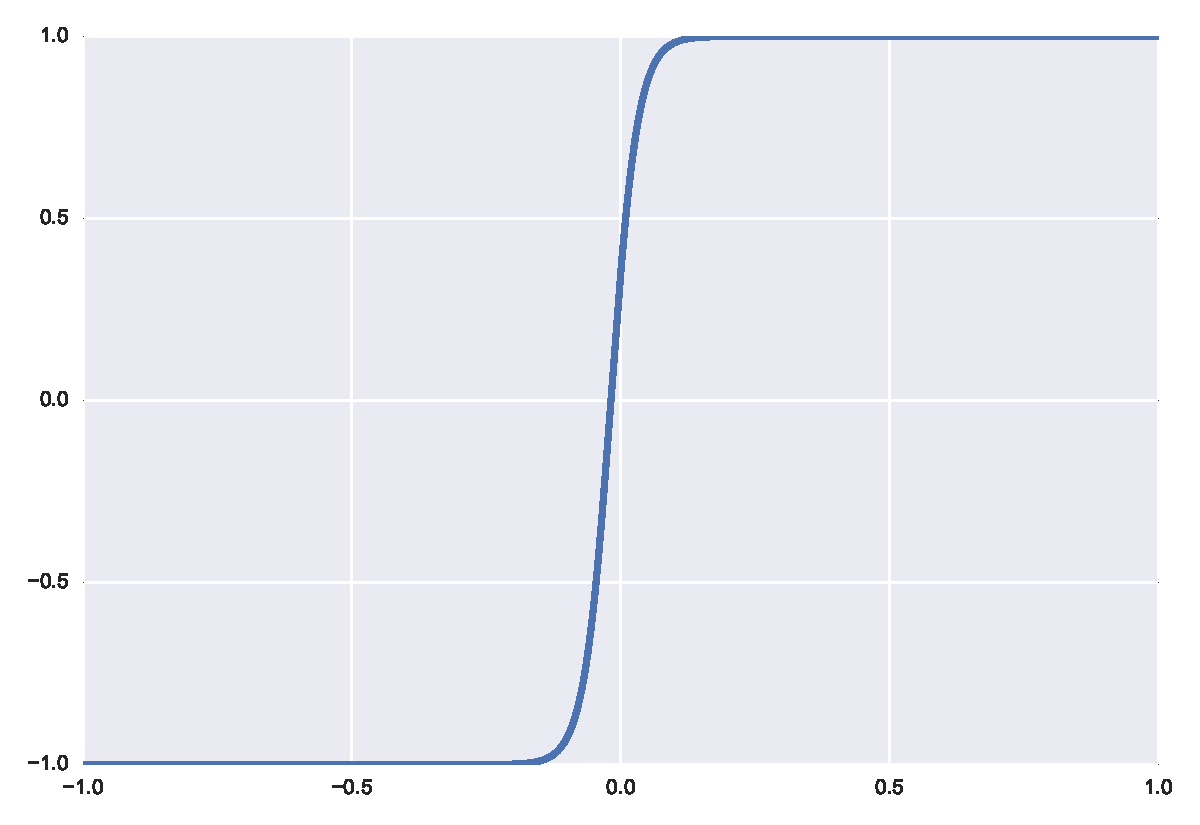
\includegraphics[width=0.7\textwidth]{/h1/dsondak/Research-Notebook/figures/2016/July/burgers_shock.pdf}
  \caption{Illustration of \fenics solution to the steady Burger's equation~\eqref{eq:burgers} using $5000$ finite elements.}
  \label{fig:burgers_shock}
\end{figure}

Next, I need to figure out how to introduce the stabilization parameter into
\fenics.  I'll base this off of Umberto's \fenics implementation of the
stabilization parameter.  Once the stabilization parameter is working, I can 
code up the magnetic field equation, followed by the nondiagonal stabilization
parameter.  Then I will introduce the nondiagonal stabilization parameter and
start compiling the results and the paper.  I will also probably need to
test everything on a two-dimensional problem.  We know that Hartmann flow
doesn't work great.  I'll have to think of another one.

\labday{Tuesday, 19 July, 2016}

\experiment{Combustion Model Inadequacy}
Nearing the end of the calibration of the reduced model.  The hold-up has been invalidating the
reduced model.  The latest results indicate that we may be able to call the calibrated
reduced model inadequate.

\subexperiment{Chemical Kinetics Inadequacy}
It would be nice to invalidate the calibrated reduced model based solely on the 0D reactor.  This has proven difficult
for the five reaction reduced model (see discussion below).  I have tried to invalidate the model with a four
reaction reduced model by removing the three-body reaction.  The algorithmic peformance is much improved (rejection
rates of around $79\%$) and chains that appear stationary.  Figures~\ref{fig:chain_1}-\ref{fig:chain_4} present
the chains from each of the four reactions.
\begin{figure}[h!]
  \centering
  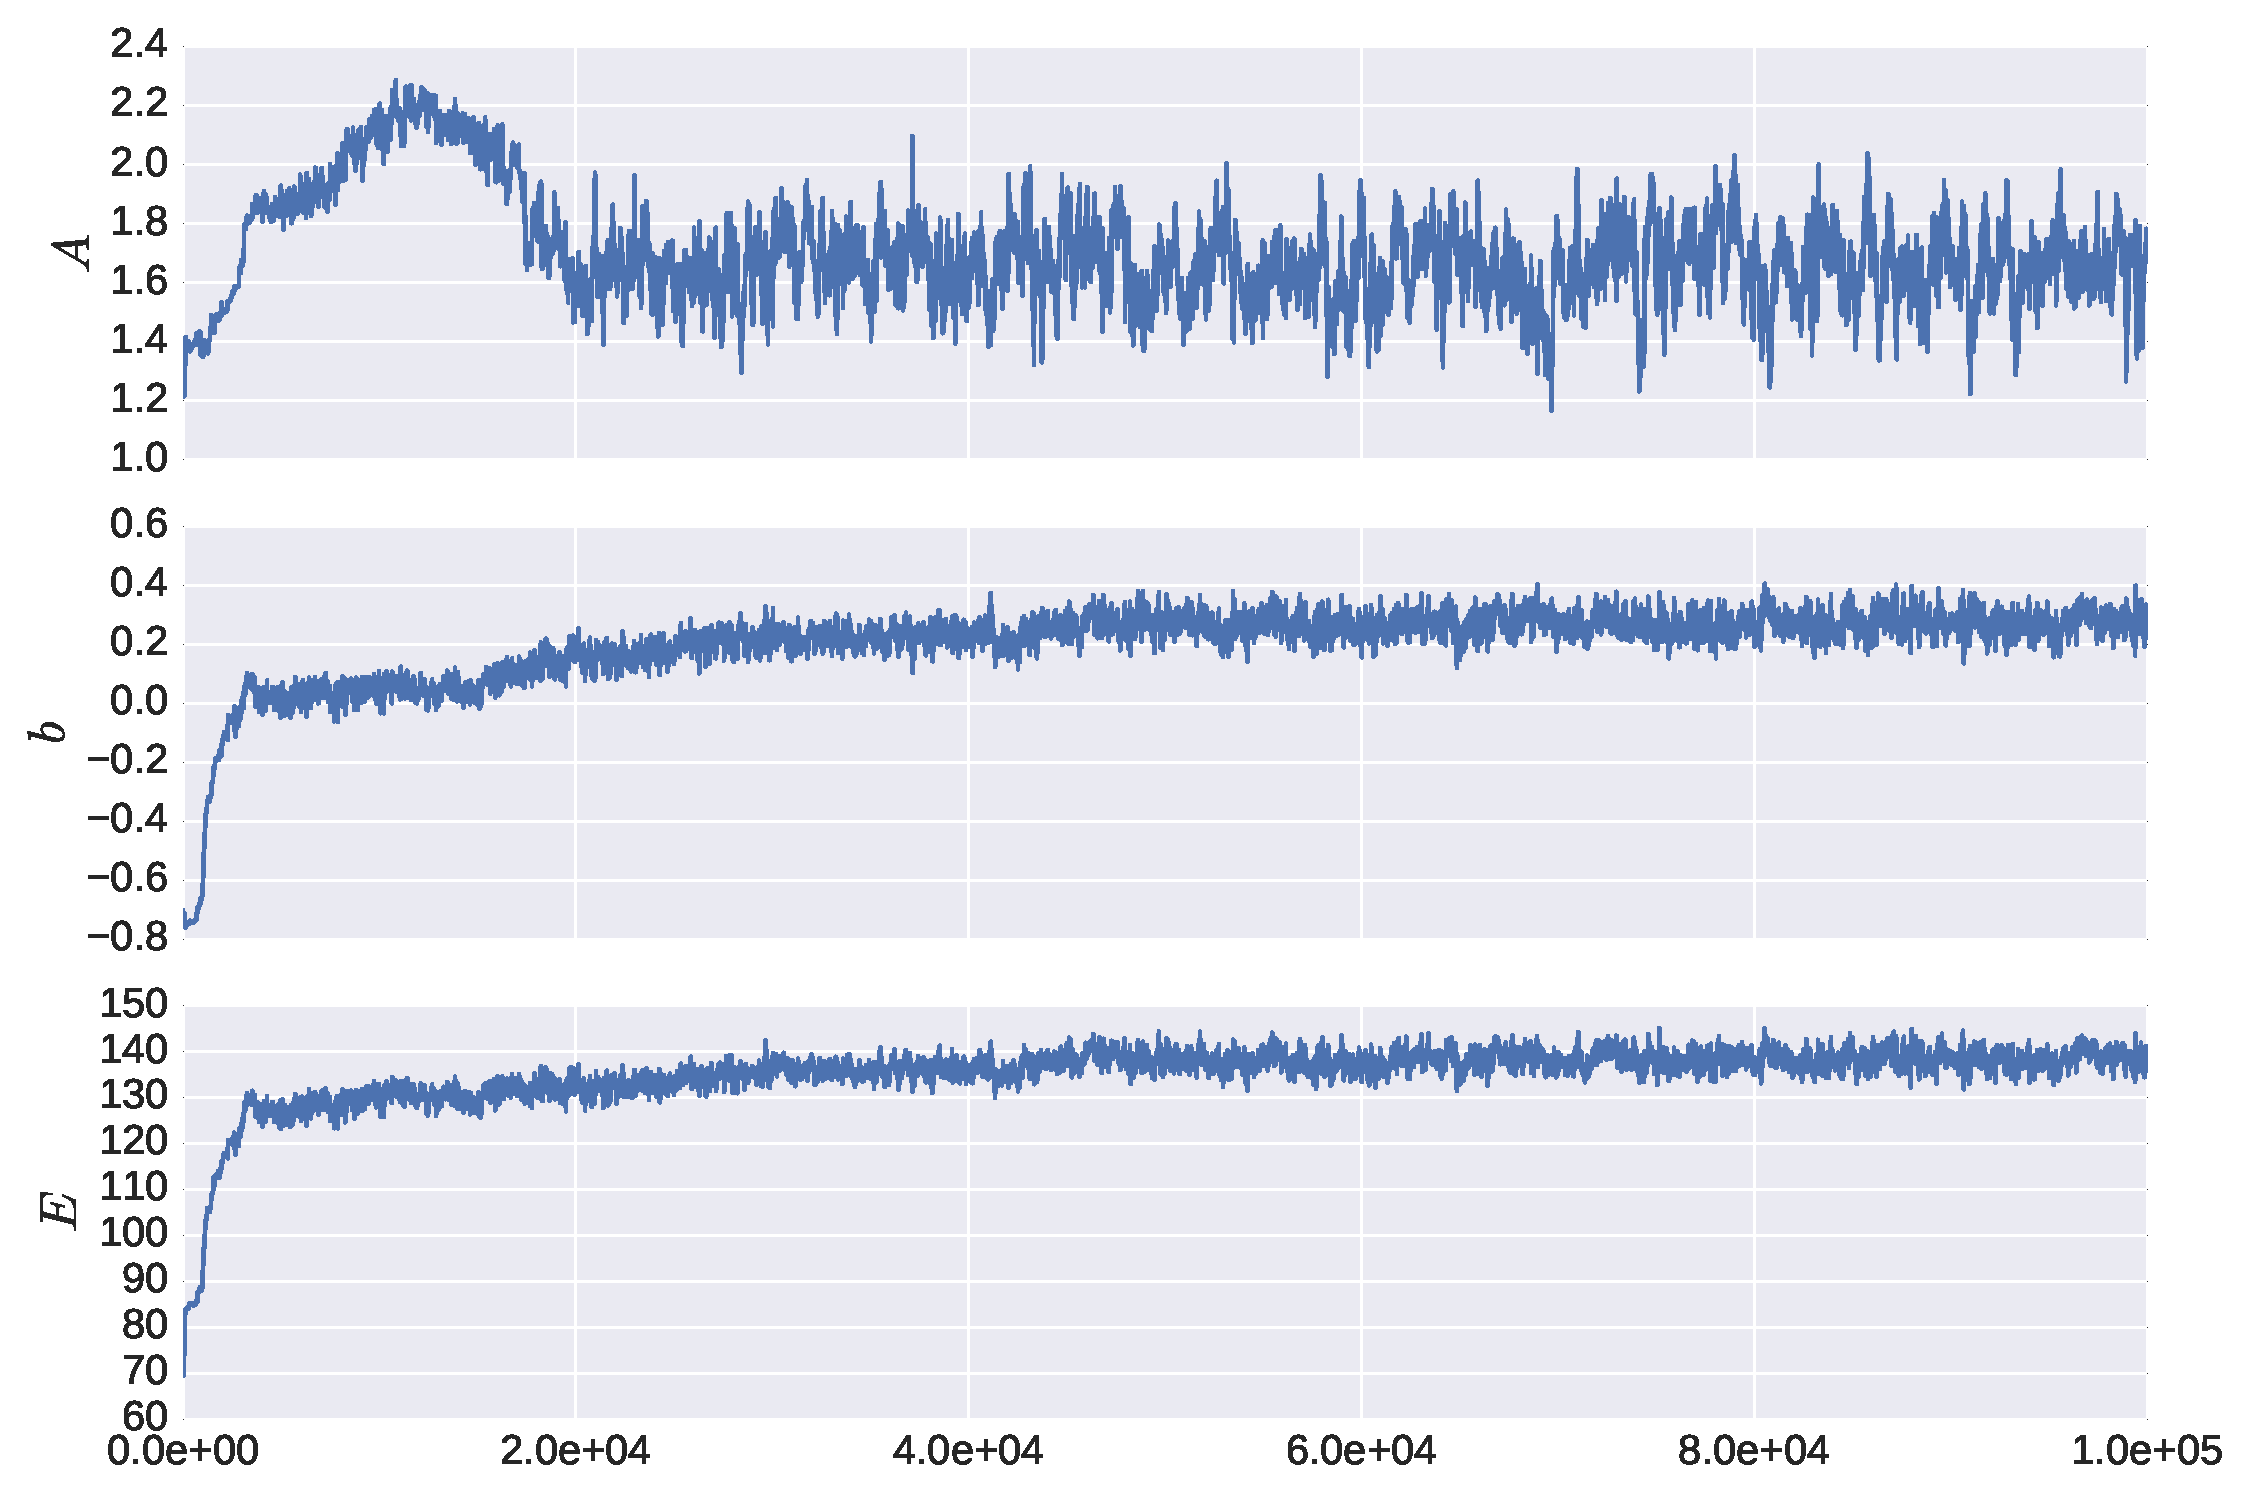
\includegraphics[width=0.7\textwidth]{/h1/dsondak/Research-Notebook/figures/2016/July/reaction0_chain.pdf}
  \caption{Chains from the calibrated Arrhenius parameters for reaction 1.}
  \label{fig:chain_1}
\end{figure}
\begin{figure}[h!]
  \centering
  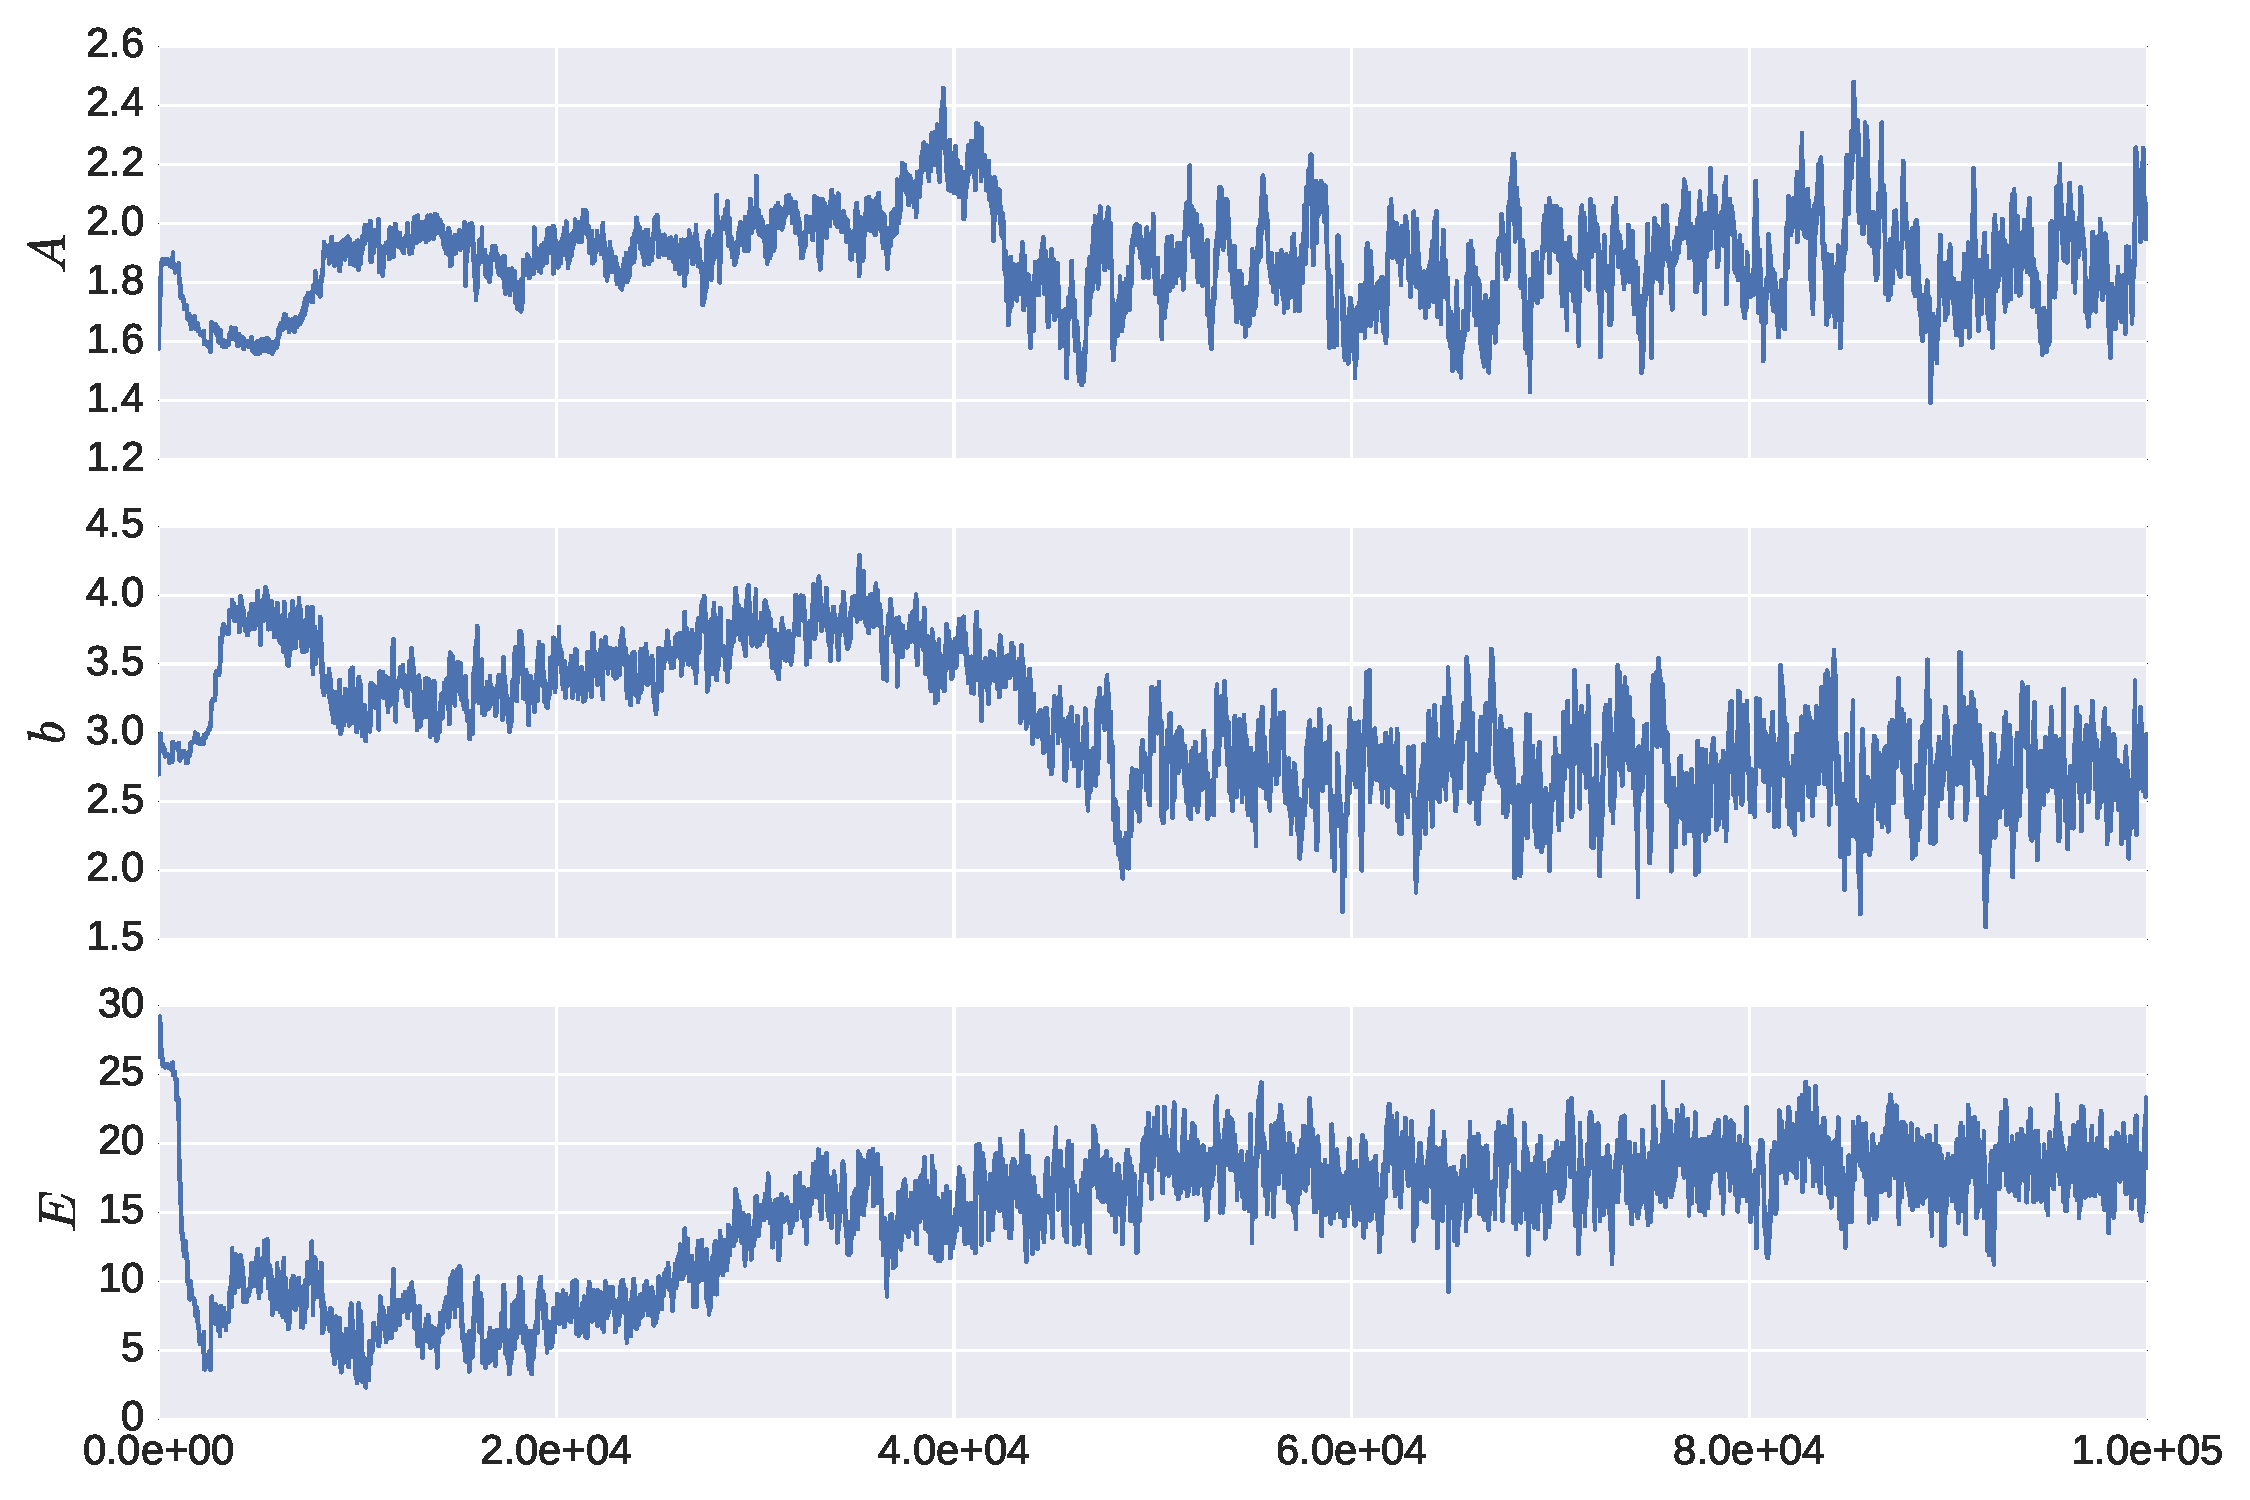
\includegraphics[width=0.7\textwidth]{/h1/dsondak/Research-Notebook/figures/2016/July/reaction1_chain.pdf}
  \caption{Chains from the calibrated Arrhenius parameters for reaction 2.  Note that the modified Arrhenius
           parameter, $b$, was frozen in the simulations even though we present a chain.}
  \label{fig:chain_2}
\end{figure}
\begin{figure}[h!]
  \centering
  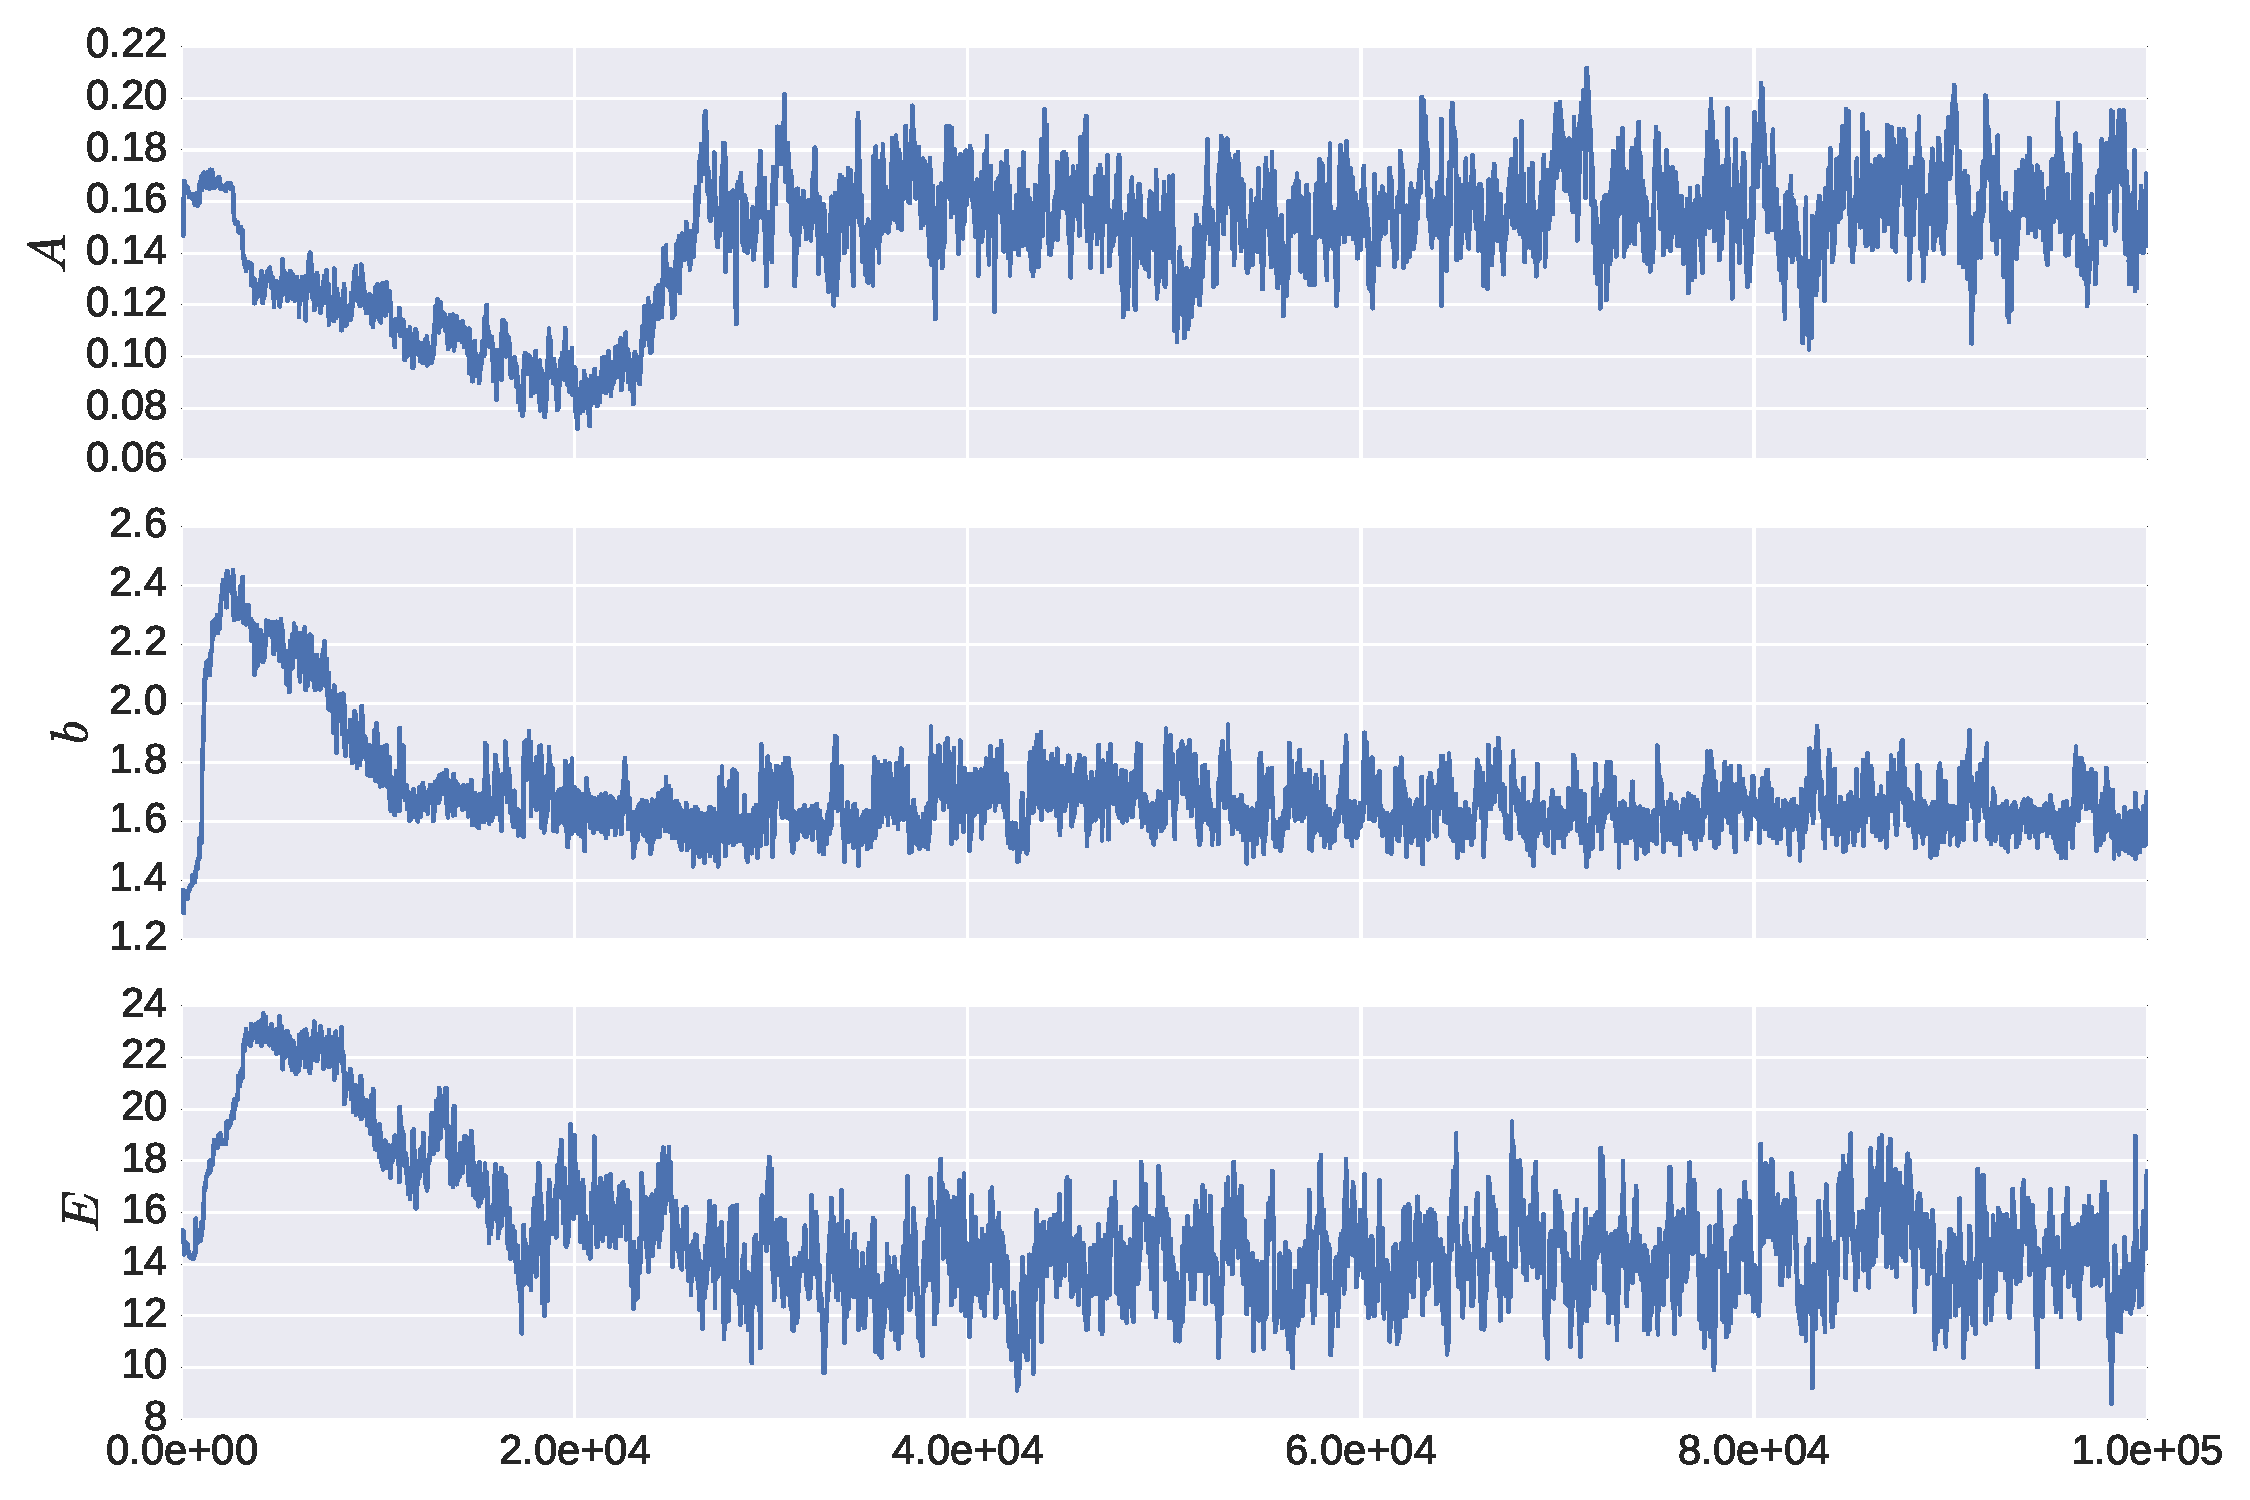
\includegraphics[width=0.7\textwidth]{/h1/dsondak/Research-Notebook/figures/2016/July/reaction2_chain.pdf}
  \caption{Chains from the calibrated Arrhenius parameters for reaction 3.}
  \label{fig:chain_3}
\end{figure}
\begin{figure}[h!]
  \centering
  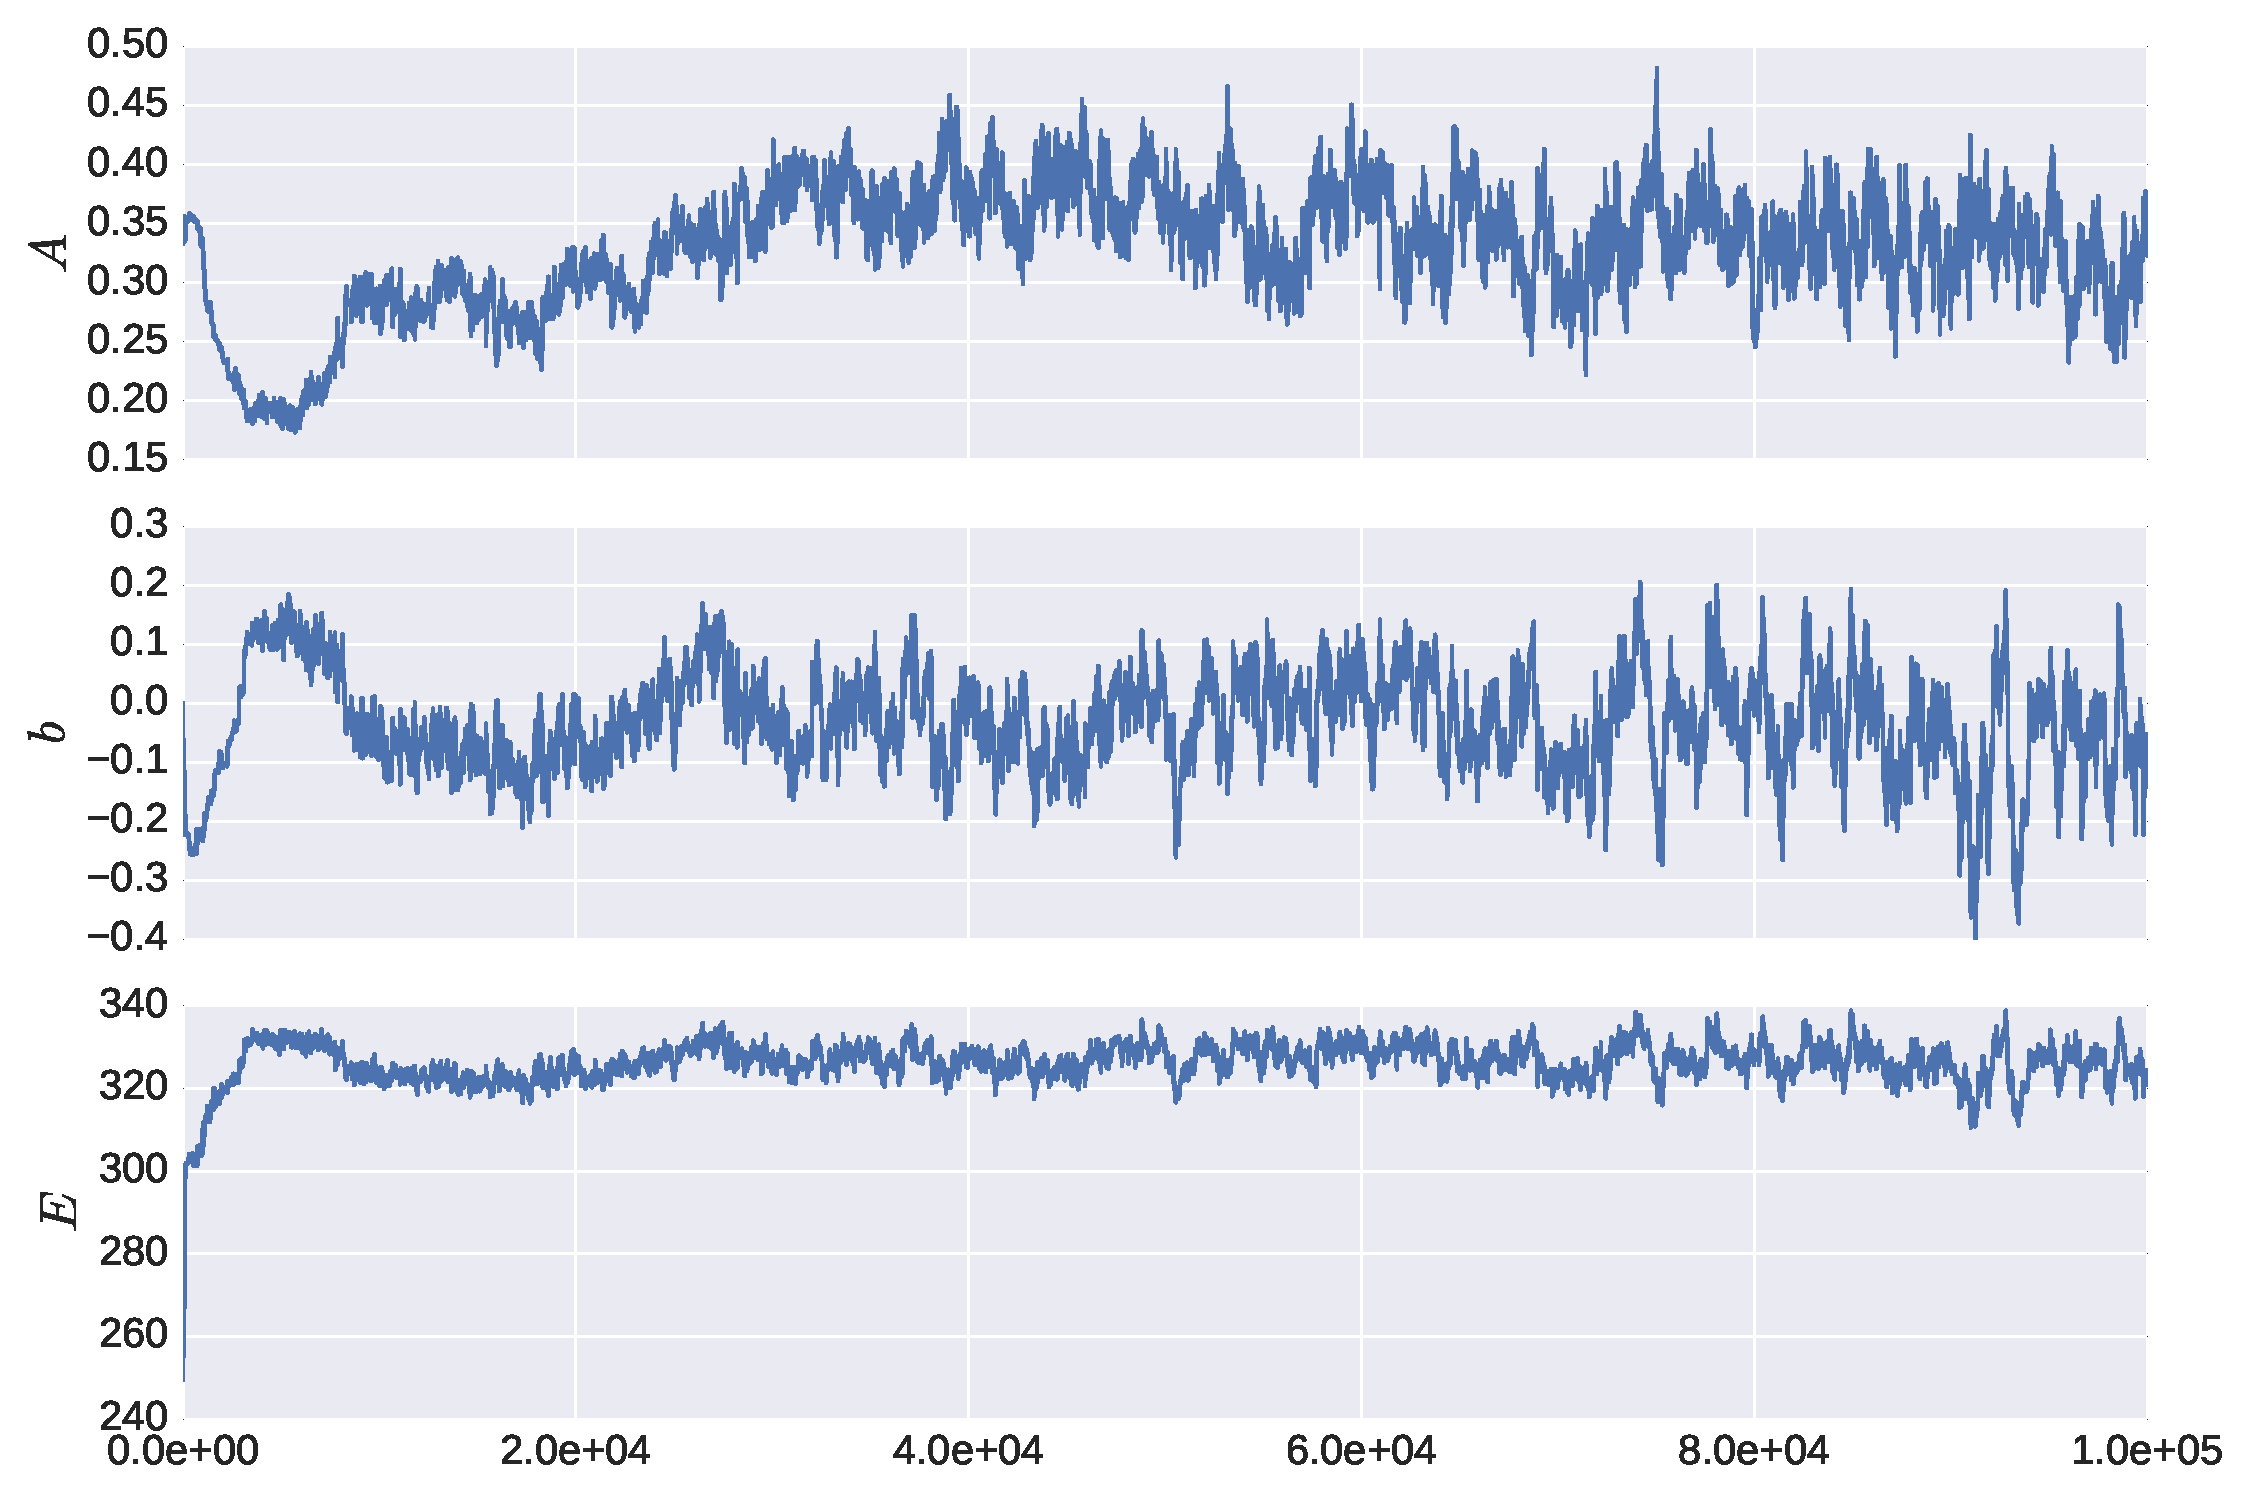
\includegraphics[width=0.7\textwidth]{/h1/dsondak/Research-Notebook/figures/2016/July/reaction3_chain.pdf}
  \caption{Chains from the calibrated Arrhenius parameters for reaction 4.}
  \label{fig:chain_4}
\end{figure}
We also provide the posterior and prior distributions for each parameter in Figures~\ref{fig:dist_1}-\ref{fig:dist_4}.  
Note that the modified Arrhenius parameter, $b$, was not actually calibrated.  It was frozen during the simulation.
\begin{figure}[h!]
  \centering
  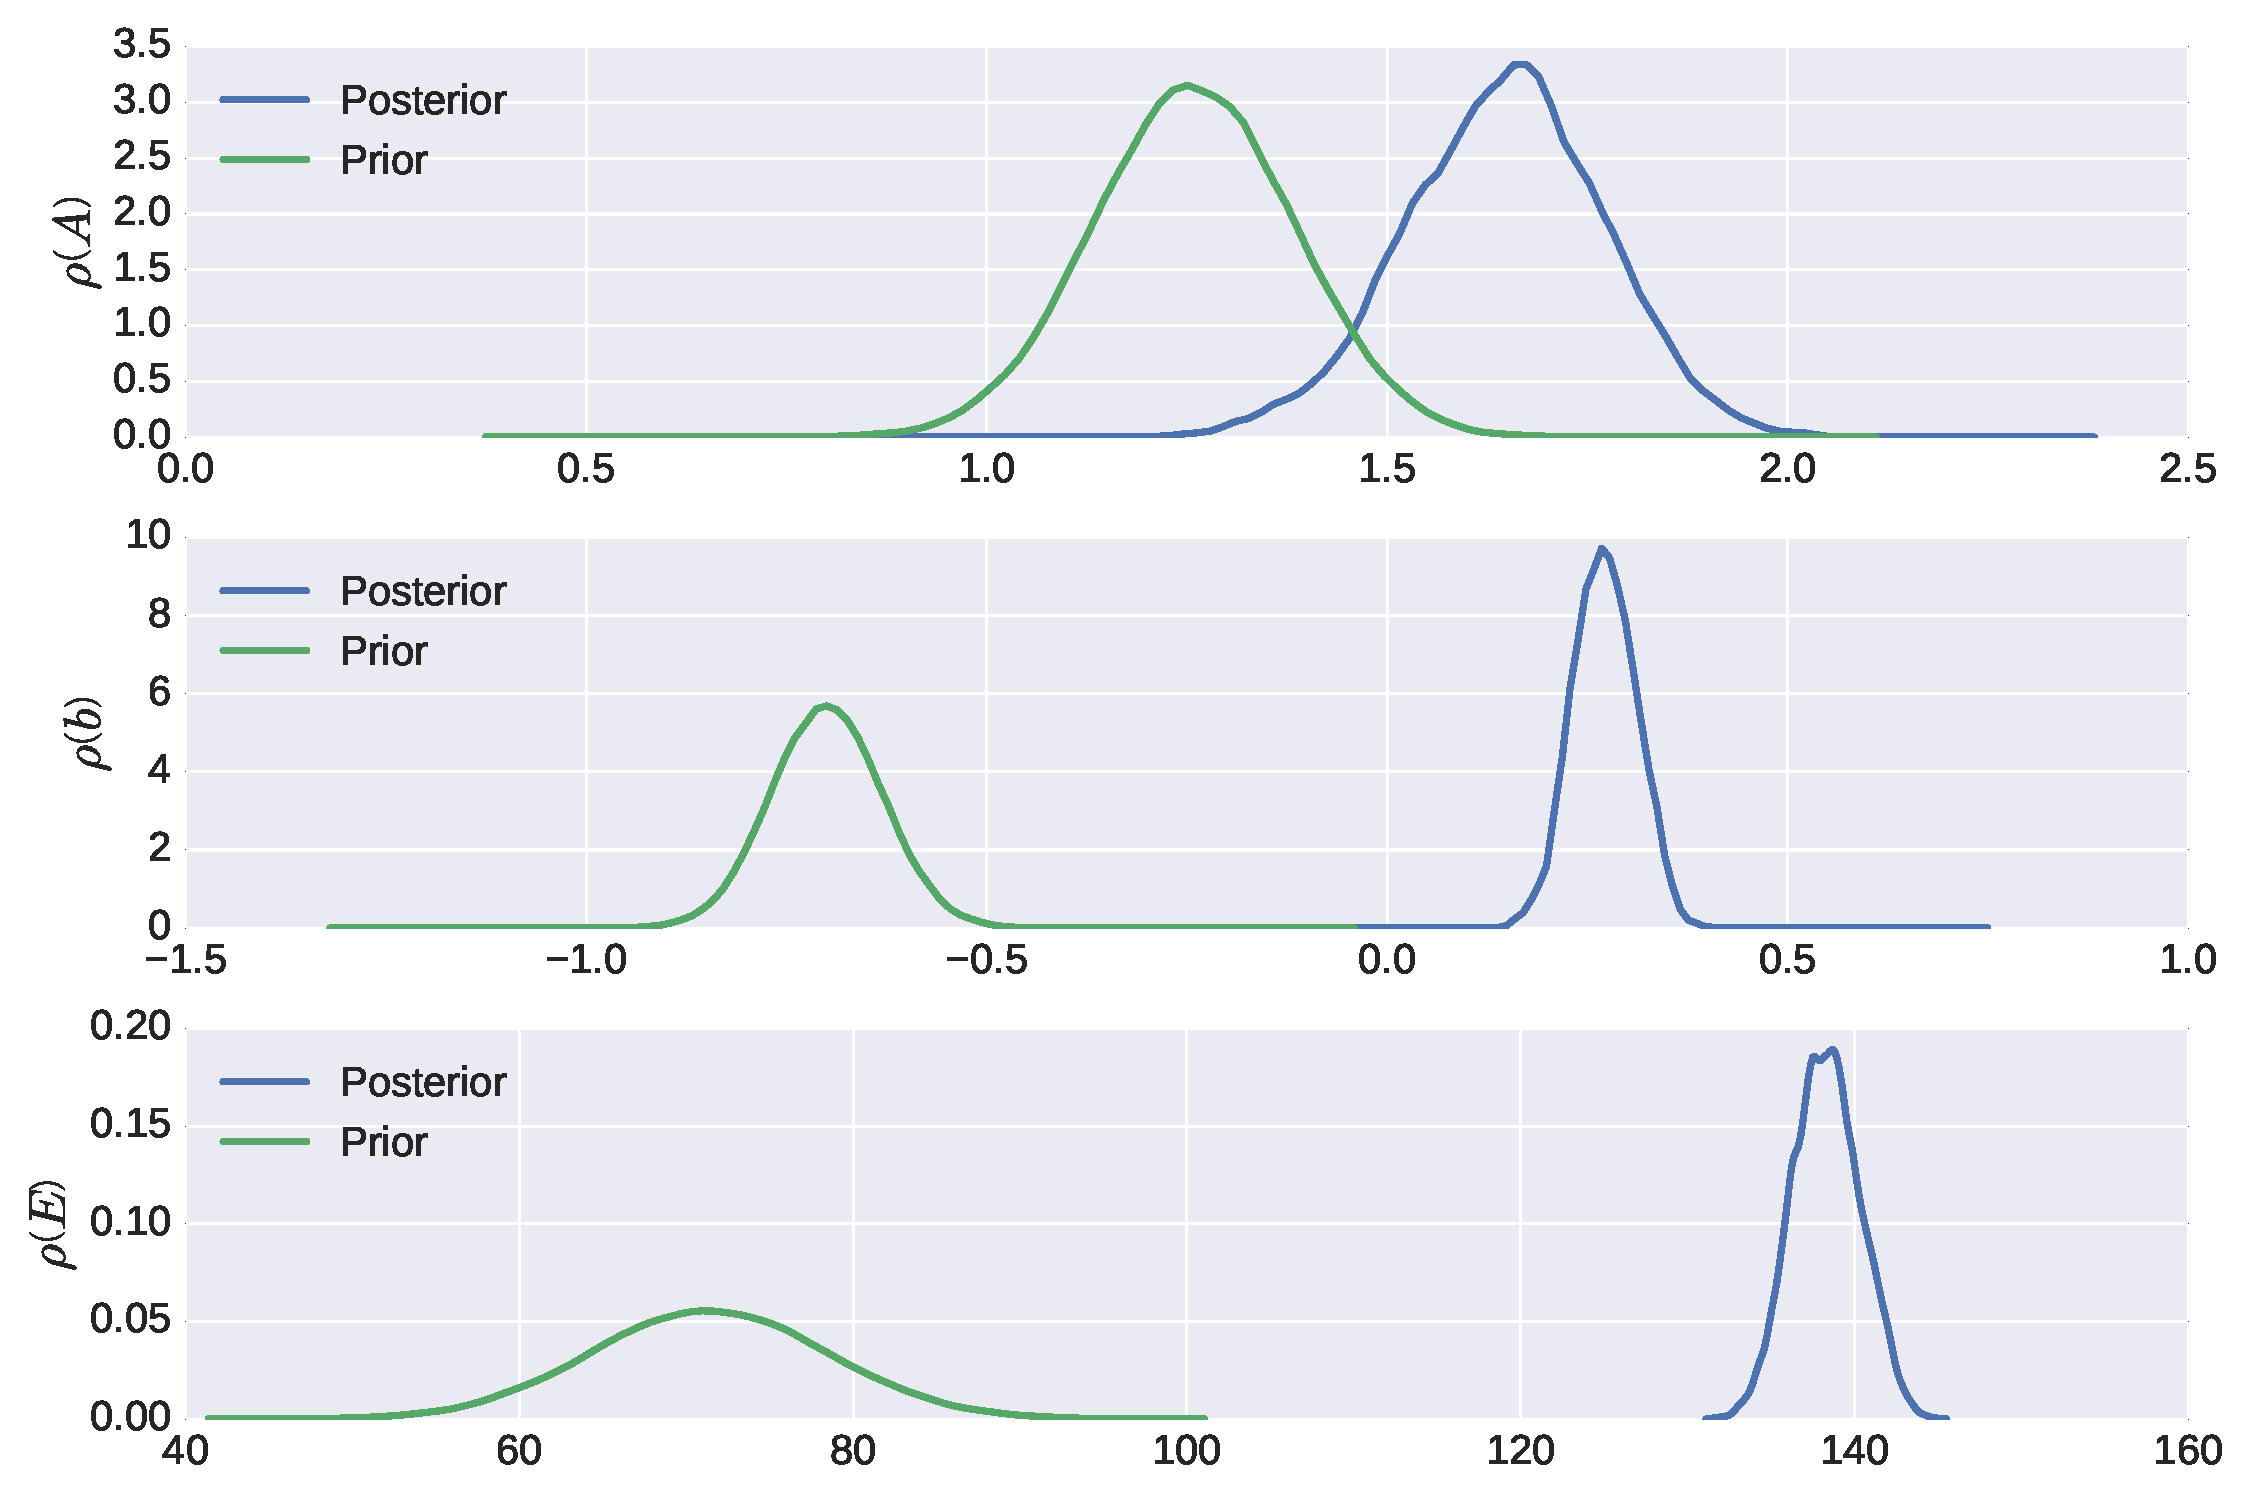
\includegraphics[width=0.7\textwidth]{/h1/dsondak/Research-Notebook/figures/2016/July/reaction0_dist.pdf}
  \caption{Posterior and prior distributions from the calibrated Arrhenius parameters for reaction 1.}
  \label{fig:dist_1}
\end{figure}
\begin{figure}[h!]
  \centering
  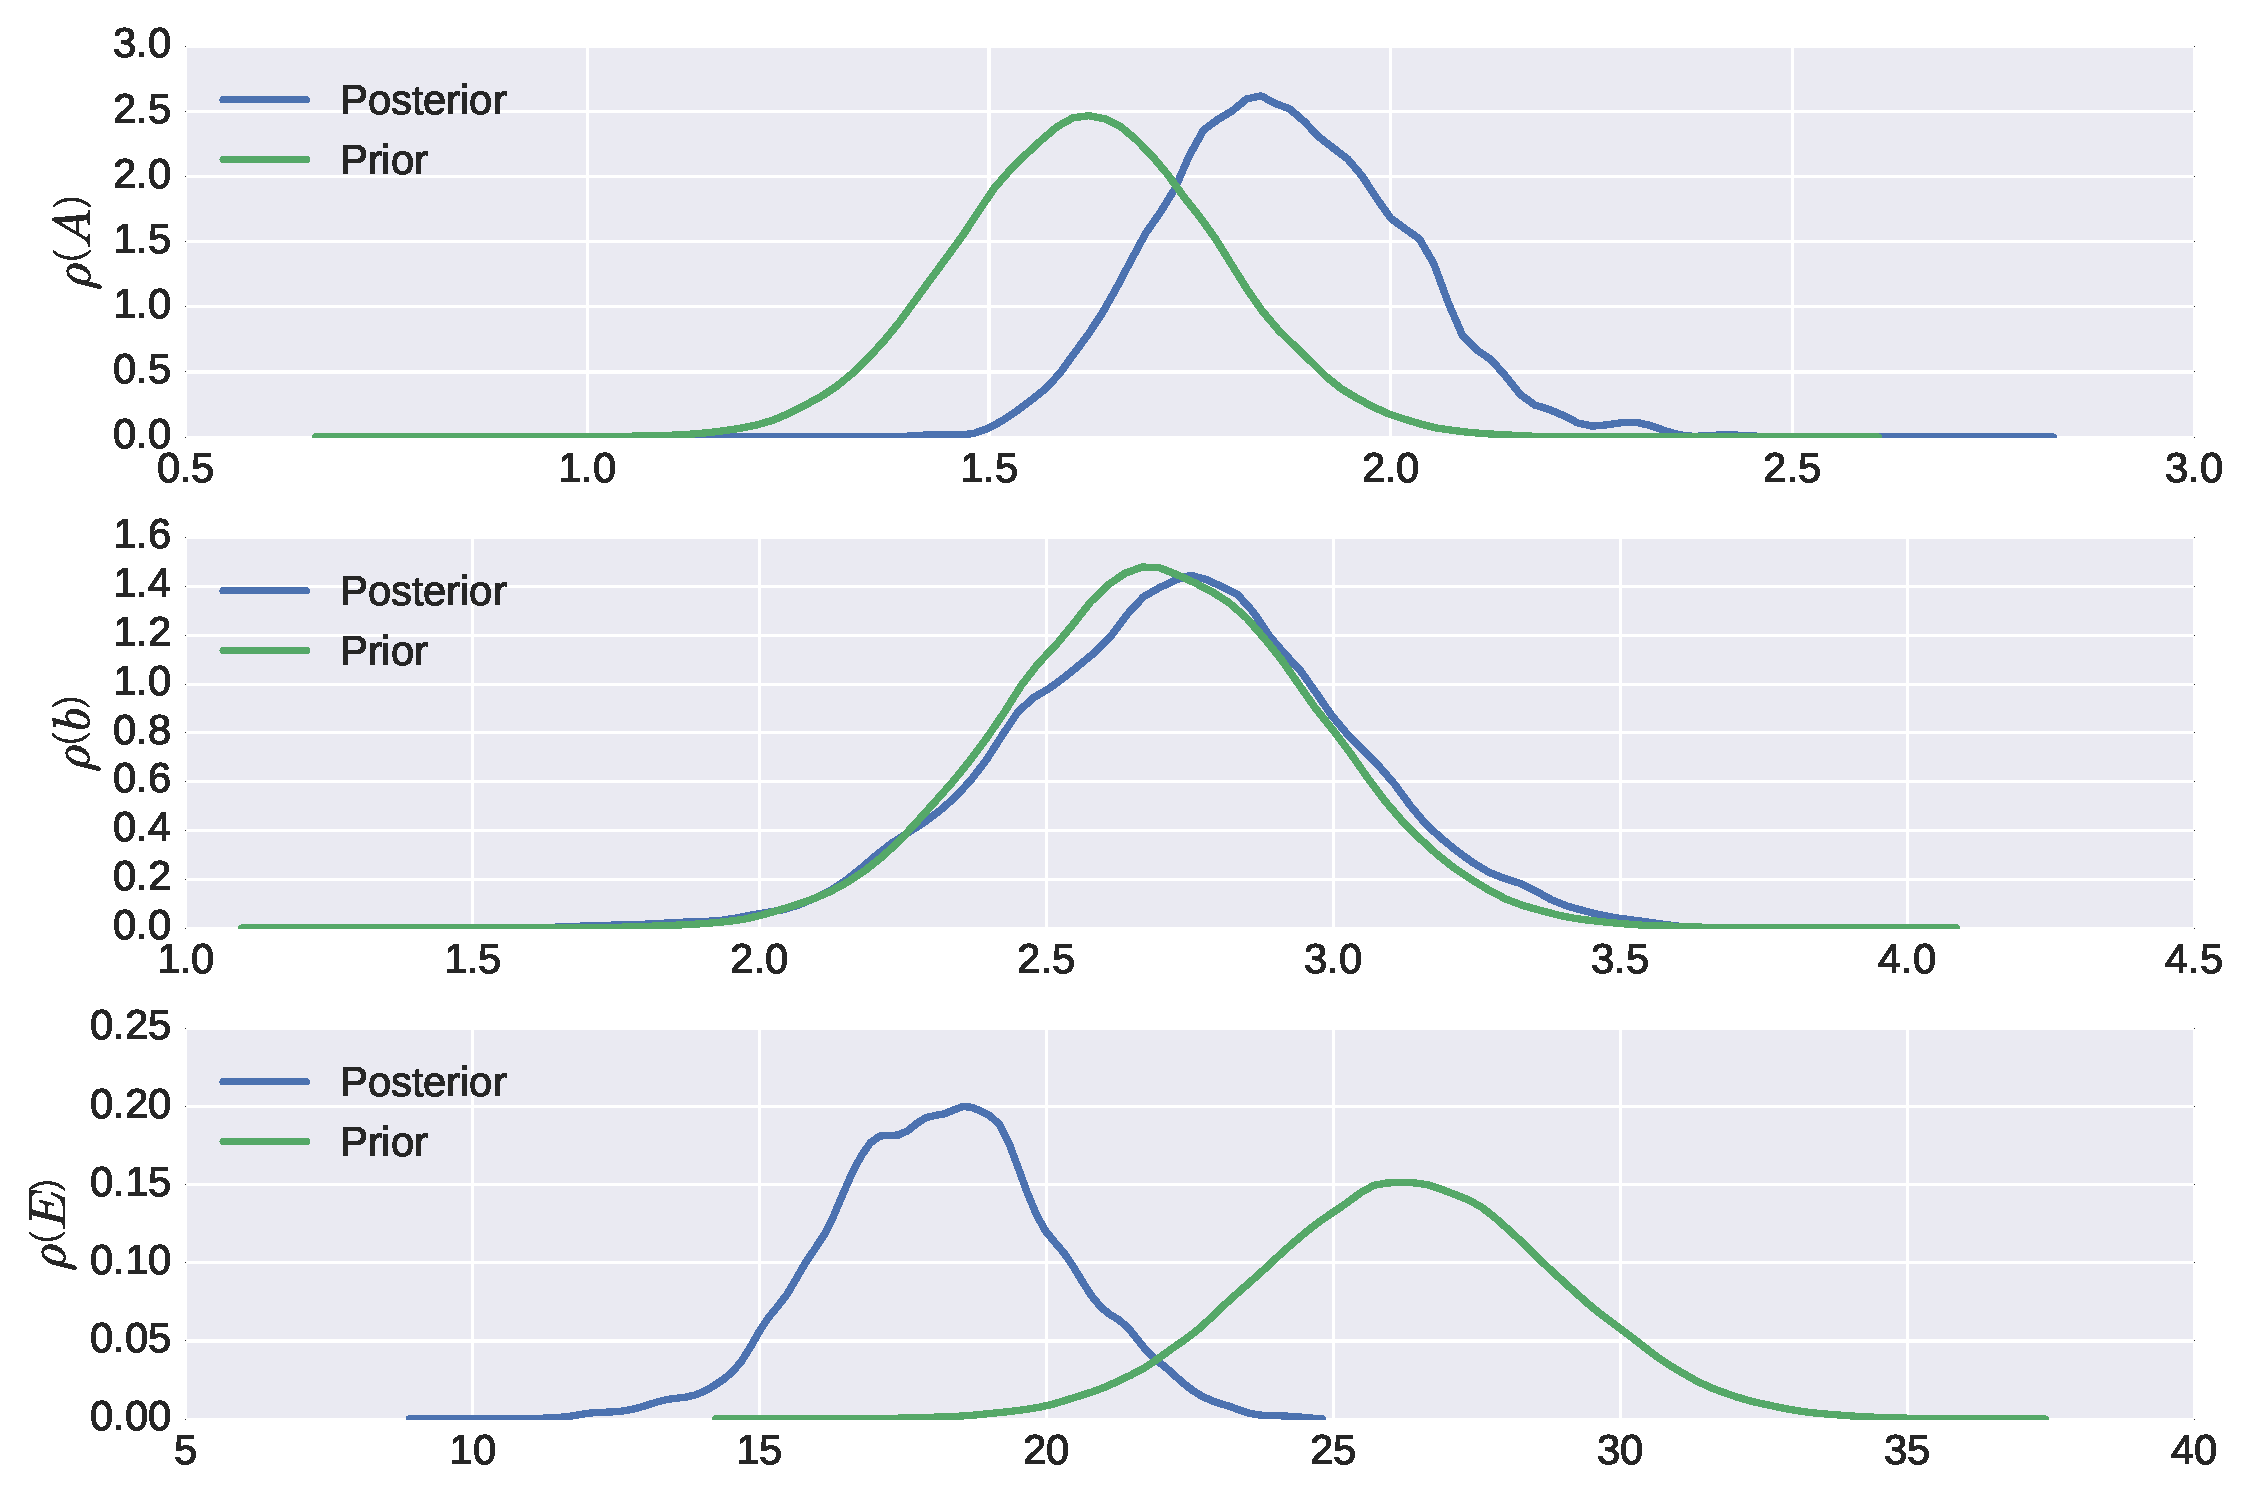
\includegraphics[width=0.7\textwidth]{/h1/dsondak/Research-Notebook/figures/2016/July/reaction1_dist.pdf}
  \caption{Posterior and prior distributions from the calibrated Arrhenius parameters for reaction 2.  Note that the modified Arrhenius
           parameter, $b$, was frozen in the simulations even though we present a chain.}
  \label{fig:dist_2}
\end{figure}
\begin{figure}[h!]
  \centering
  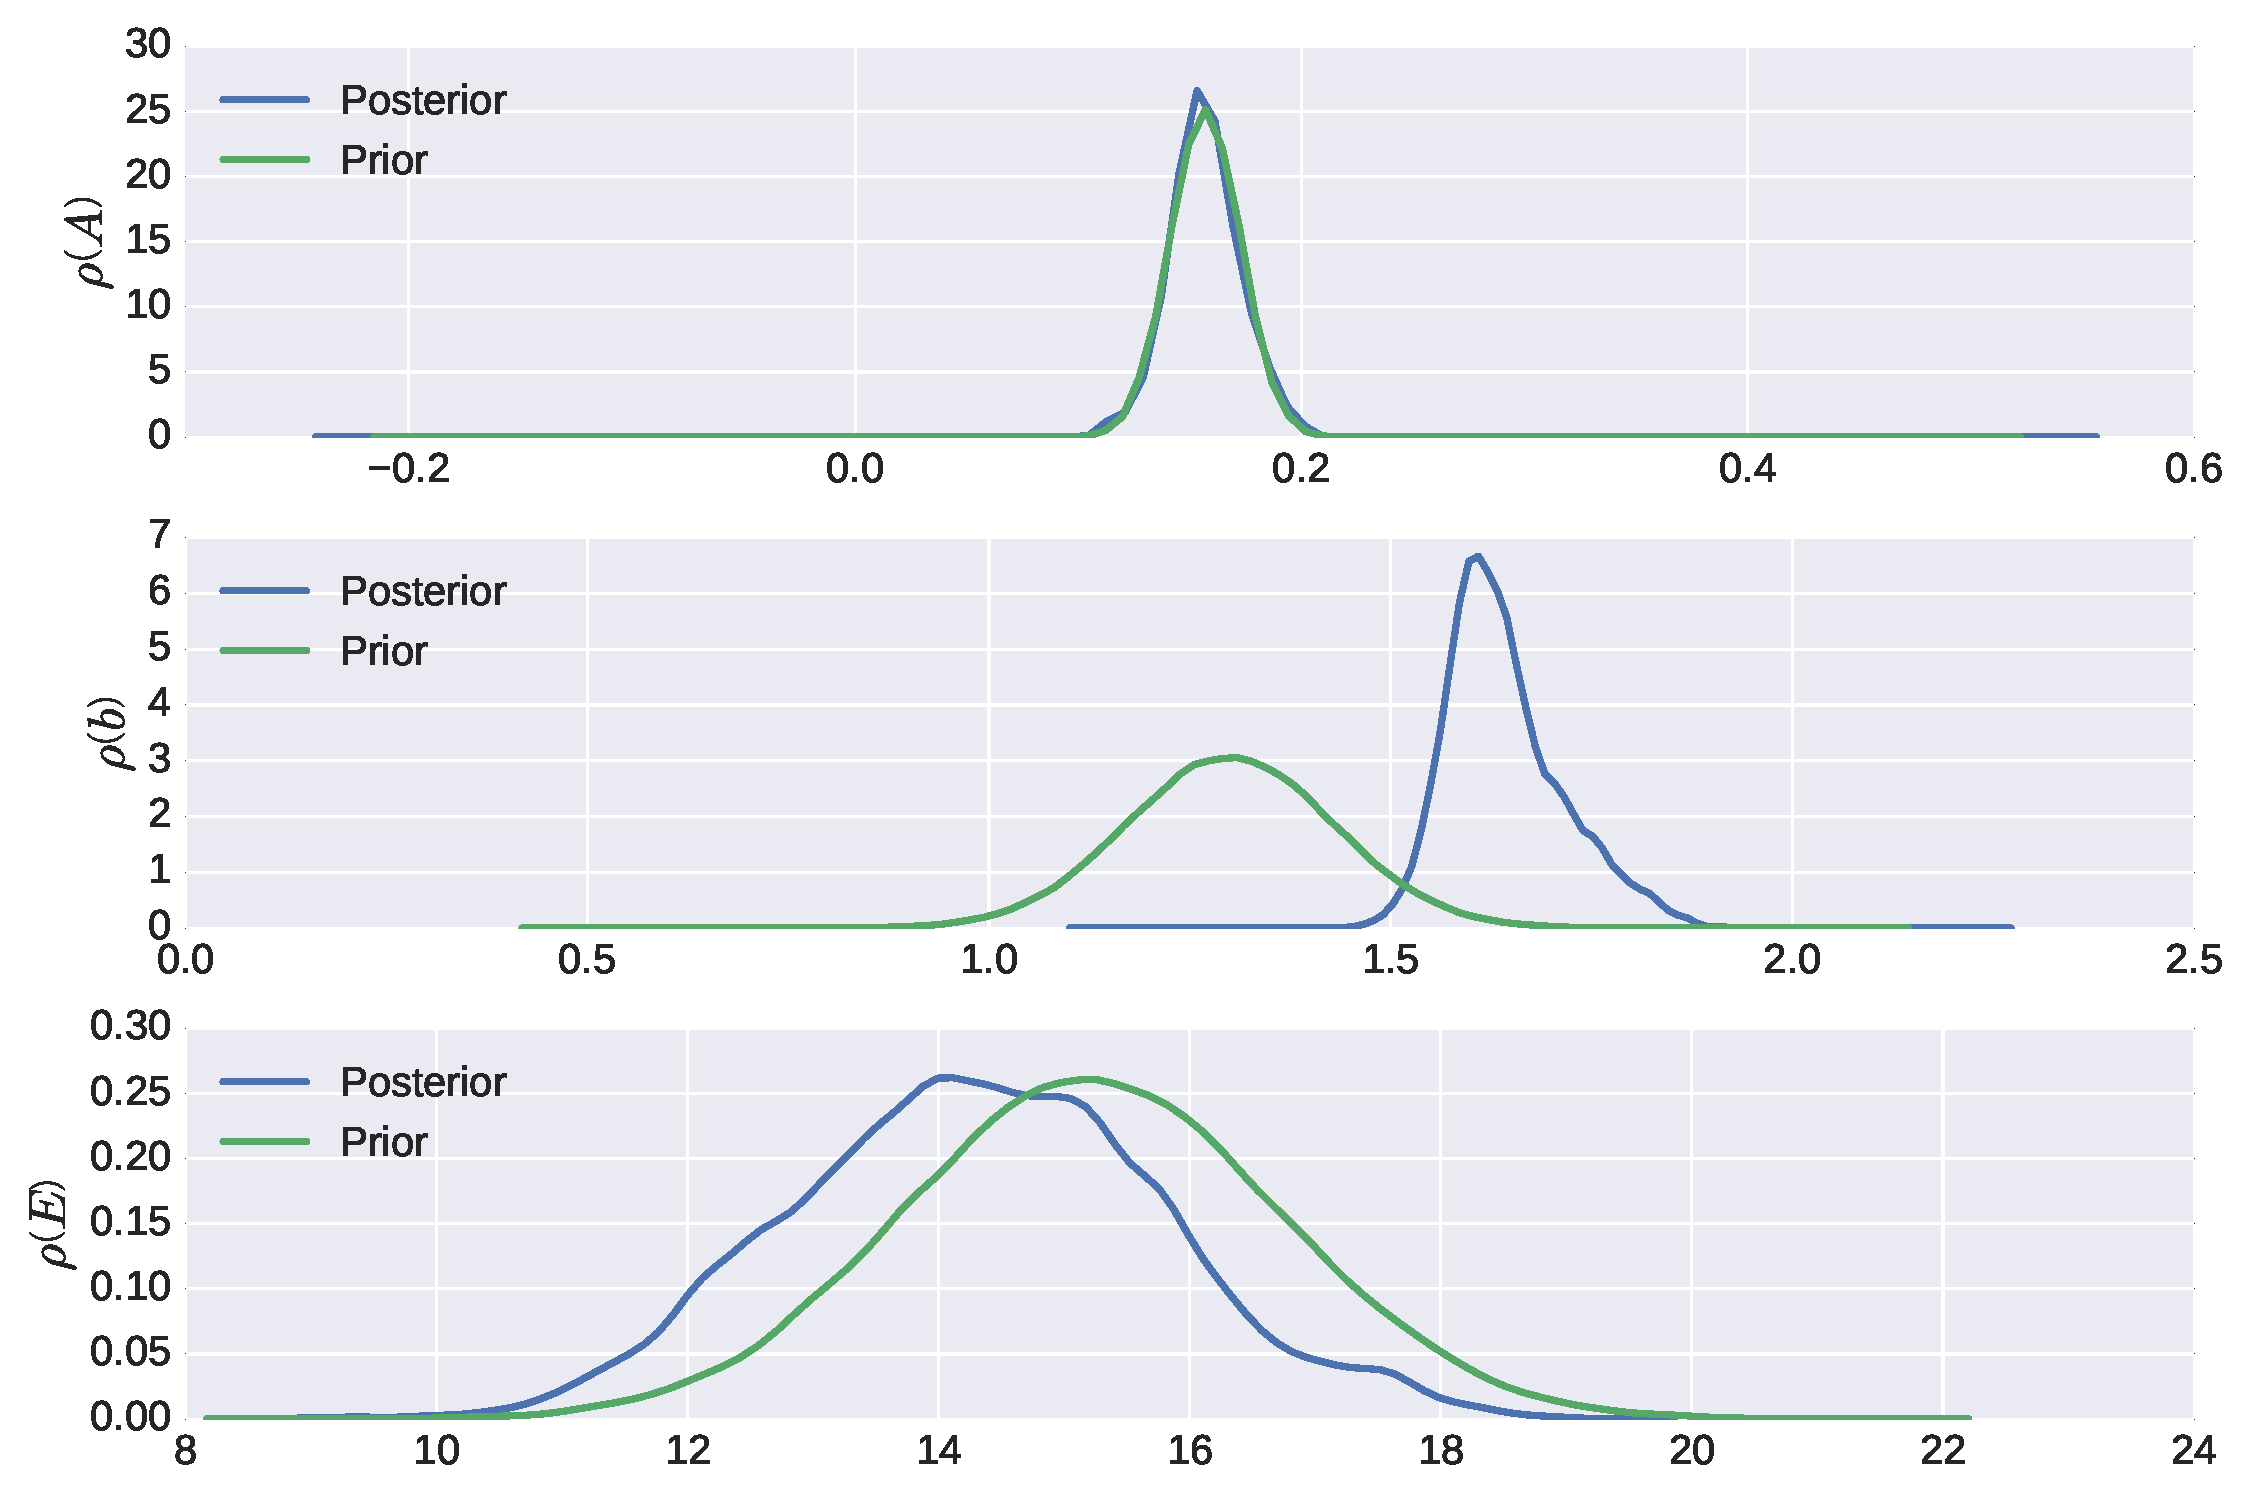
\includegraphics[width=0.7\textwidth]{/h1/dsondak/Research-Notebook/figures/2016/July/reaction2_dist.pdf}
  \caption{Posterior and prior distributions from the calibrated Arrhenius parameters for reaction 3.}
  \label{fig:dist_3}
\end{figure}
\begin{figure}[h!]
  \centering
  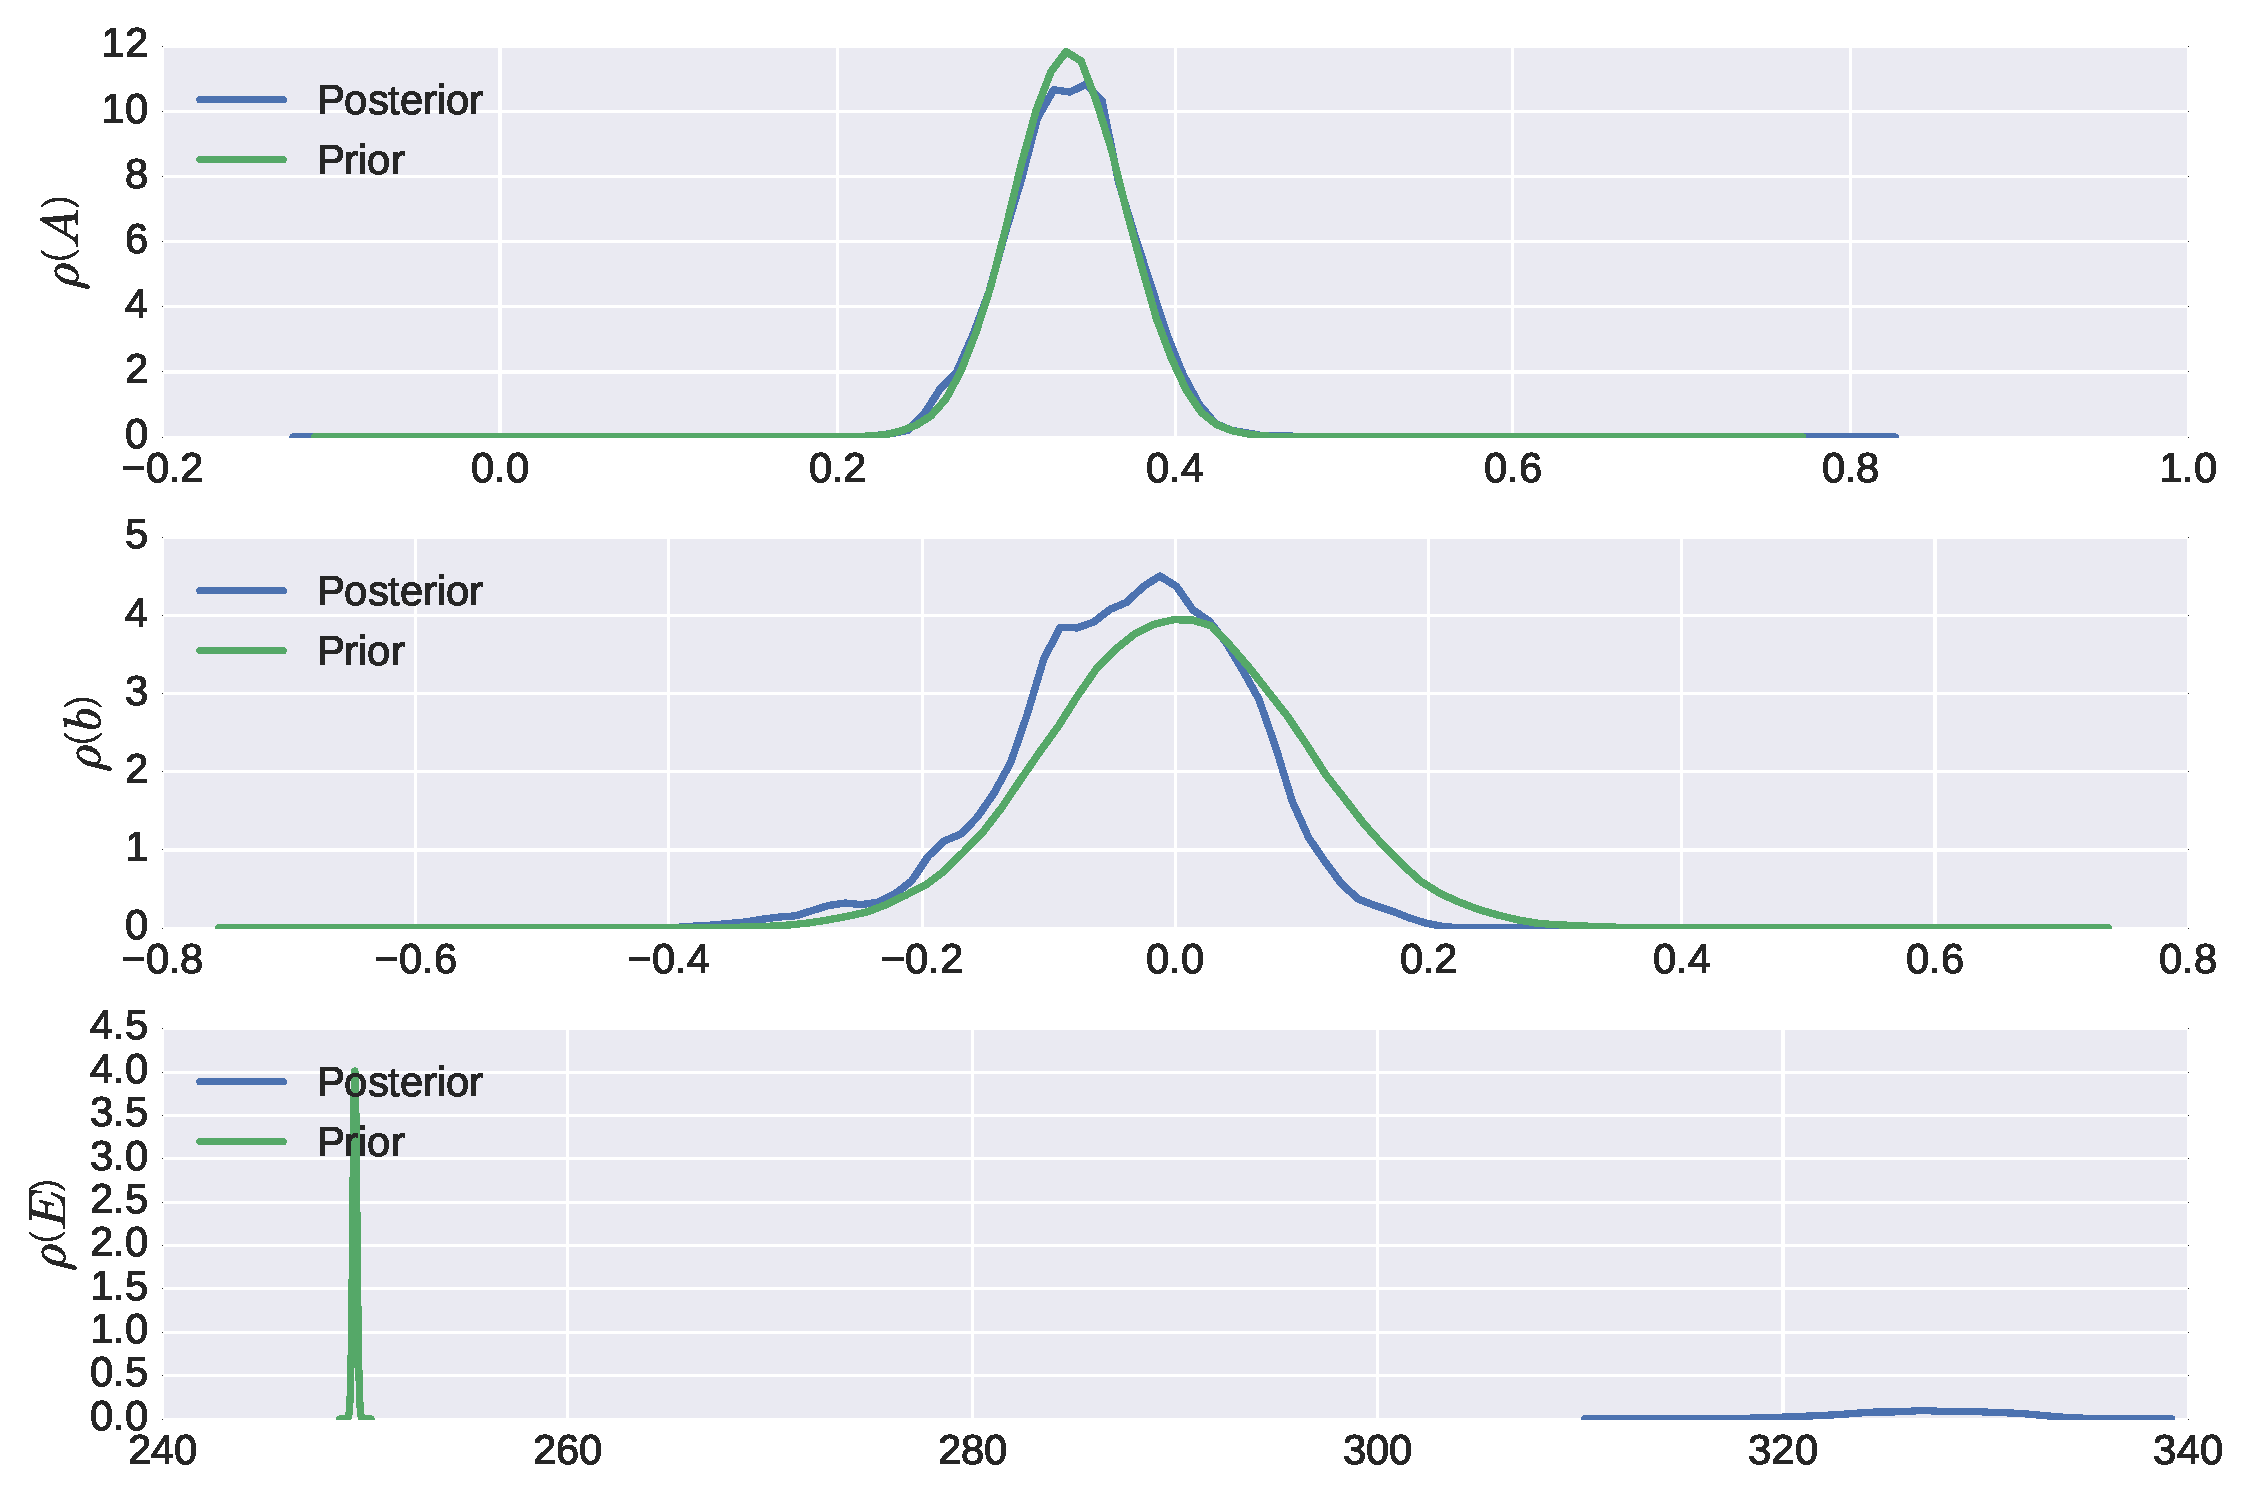
\includegraphics[width=0.7\textwidth]{/h1/dsondak/Research-Notebook/figures/2016/July/reaction3_dist.pdf}
  \caption{Posterior and prior distributions from the calibrated Arrhenius parameters for reaction 4.}
  \label{fig:dist_4}
\end{figure}
It appears that we are learning quite a bit about a few parameters.  The maximum likelihood and MAP point
were obtained from the chains and the forward problem was run at each of these parameter sets.  The 
problem was also run at the nominal parameter set.  Results were compared with the detailed model and are
shown in Figure~\ref{fig:four_rxn_inad}.
\begin{figure}[h!]
  \centering
  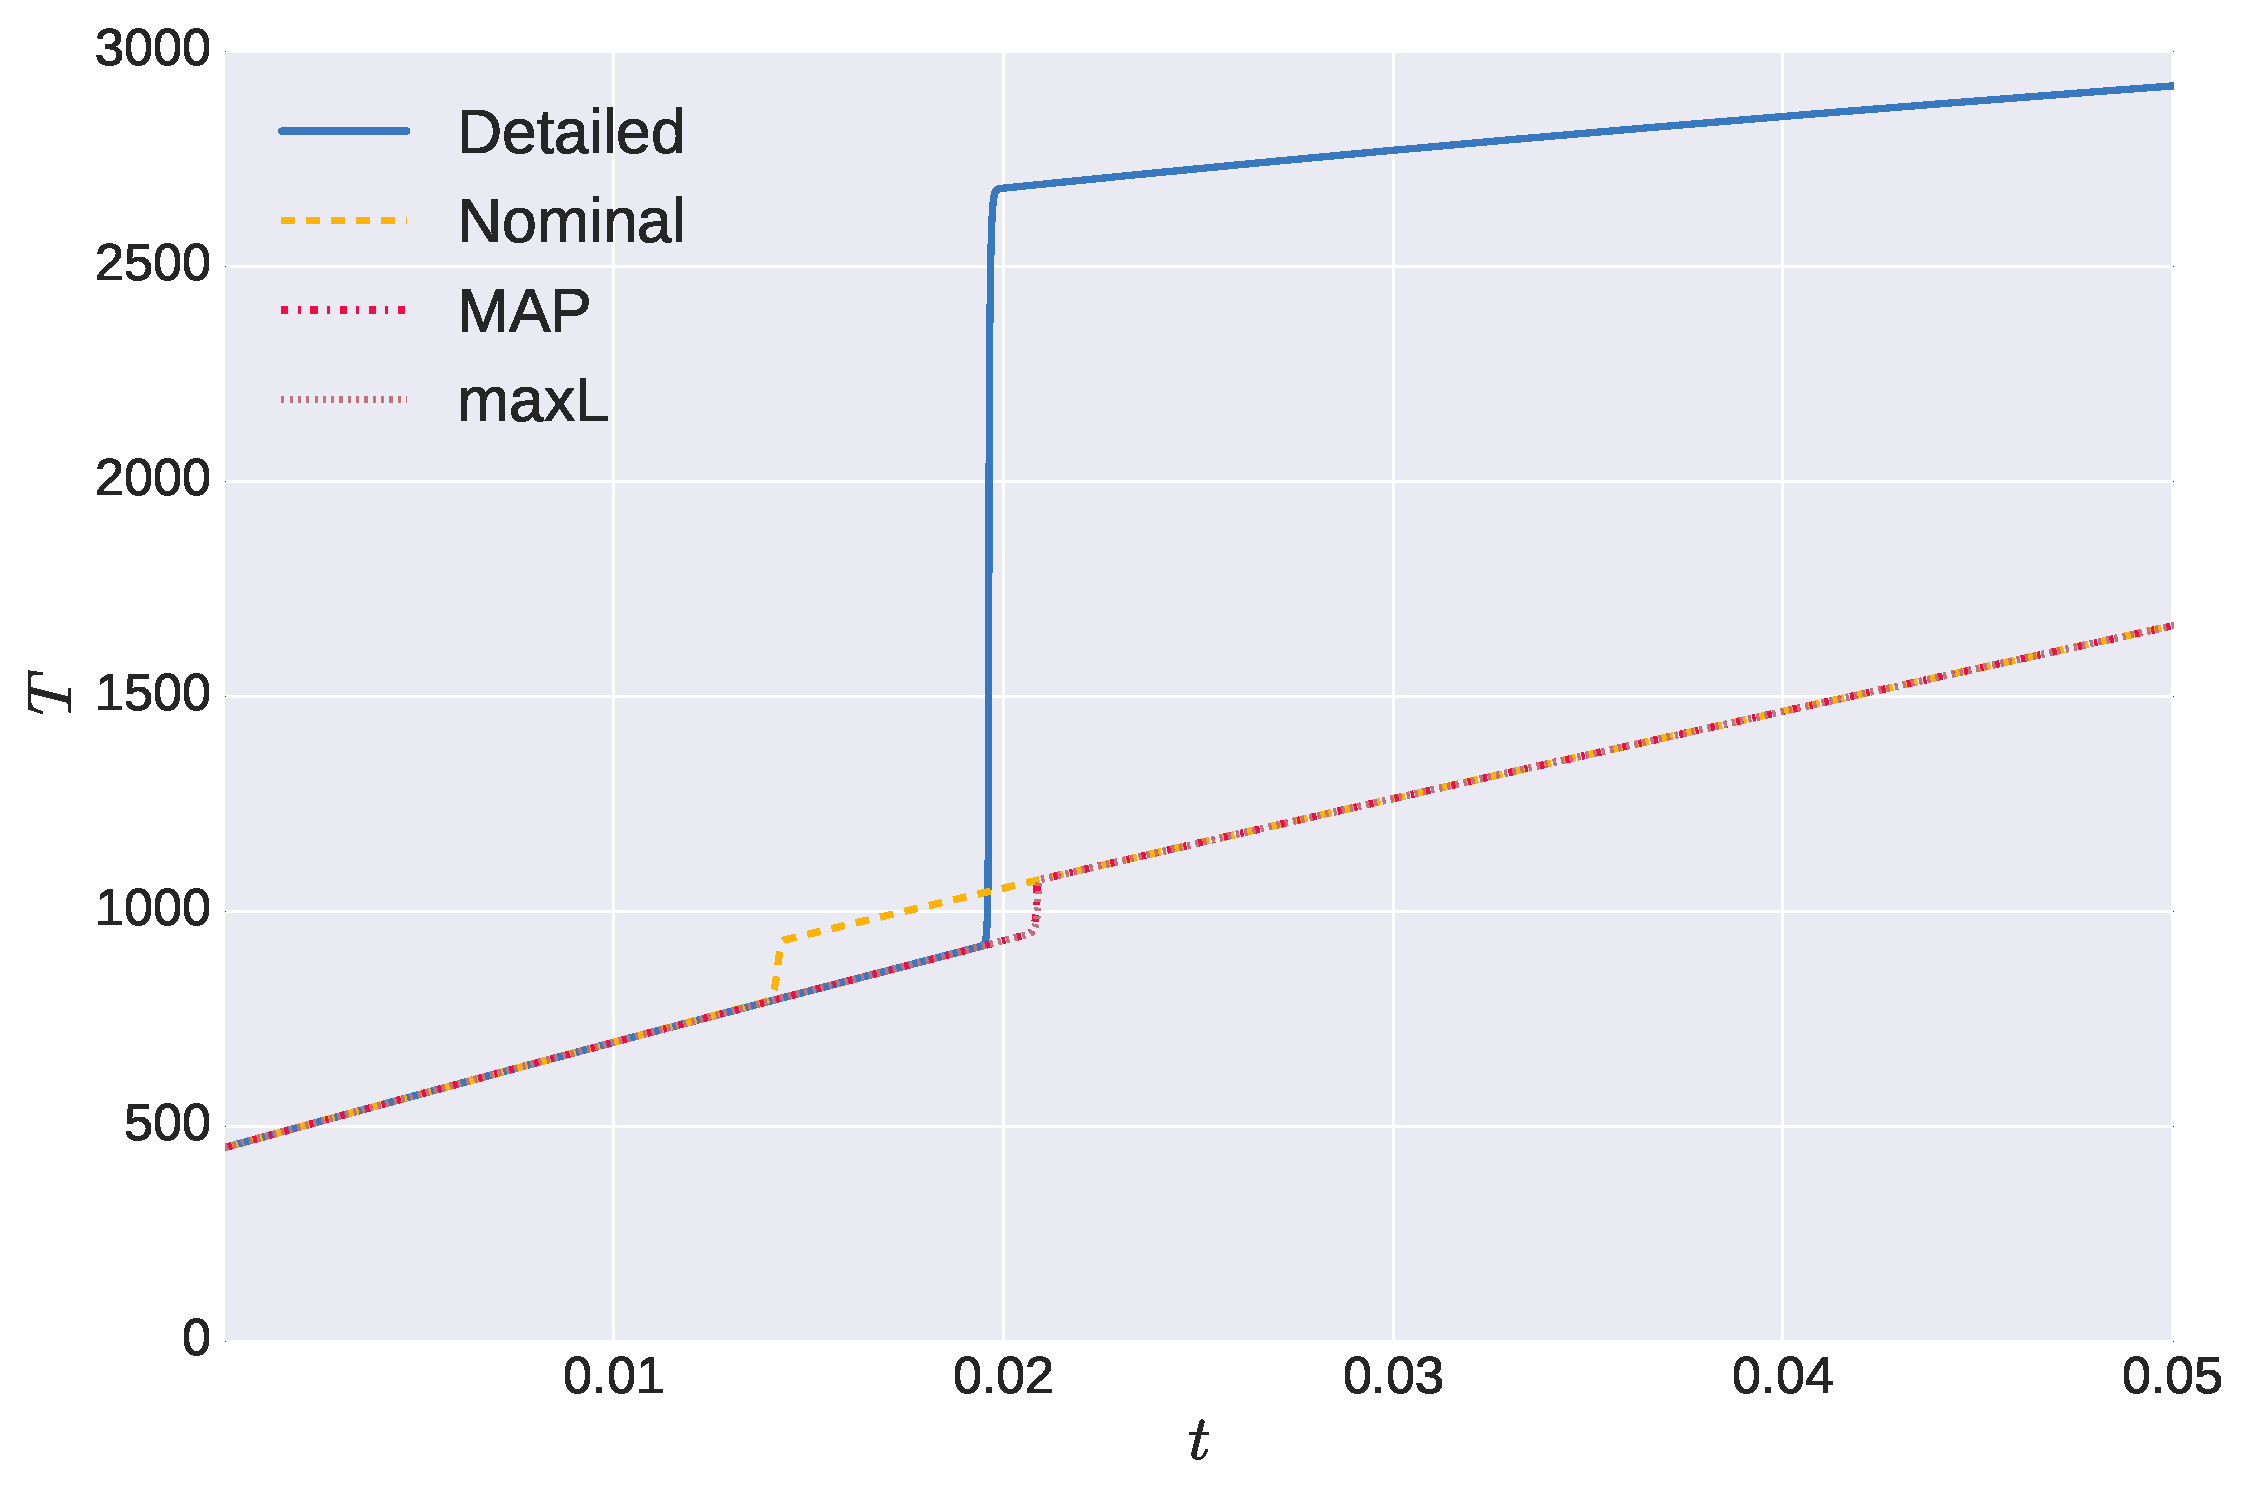
\includegraphics[width=0.7\textwidth]{/h1/dsondak/Research-Notebook/figures/2016/July/Toft_four_rxn_inad.pdf}
  \caption{Time evolution of the temperature.  Comparisons are made between the four reaction reduced model
           for three different parameter sets and the detailed model.  Results are shown at $\phi=1$ which
           is the equivalence ratio at which the data was calibrated.}
  \label{fig:four_rxn_inad}
\end{figure}
Even after calibration, the four reaction model is inadequate.  This may provide a simple route to helping
Rebecca get her stuff going again.  I'll need to calibrate the stochastic operator on this problem and then
see how things look.  For now, I need to get the stochastic operator up and running.

\subexperiment{Diffusion Flame}
The diffusion flame will eventually be used to build up a flamelet library.  For now, I'm just using it to
see if it helps us invalidate the five reaction reduced mechanism.  Figures~\ref{fig:T_Z}-\ref{fig:H2_x} were generated
from samples of the five reaction reduced mechanism.
\begin{figure}[h!]
  \centering
  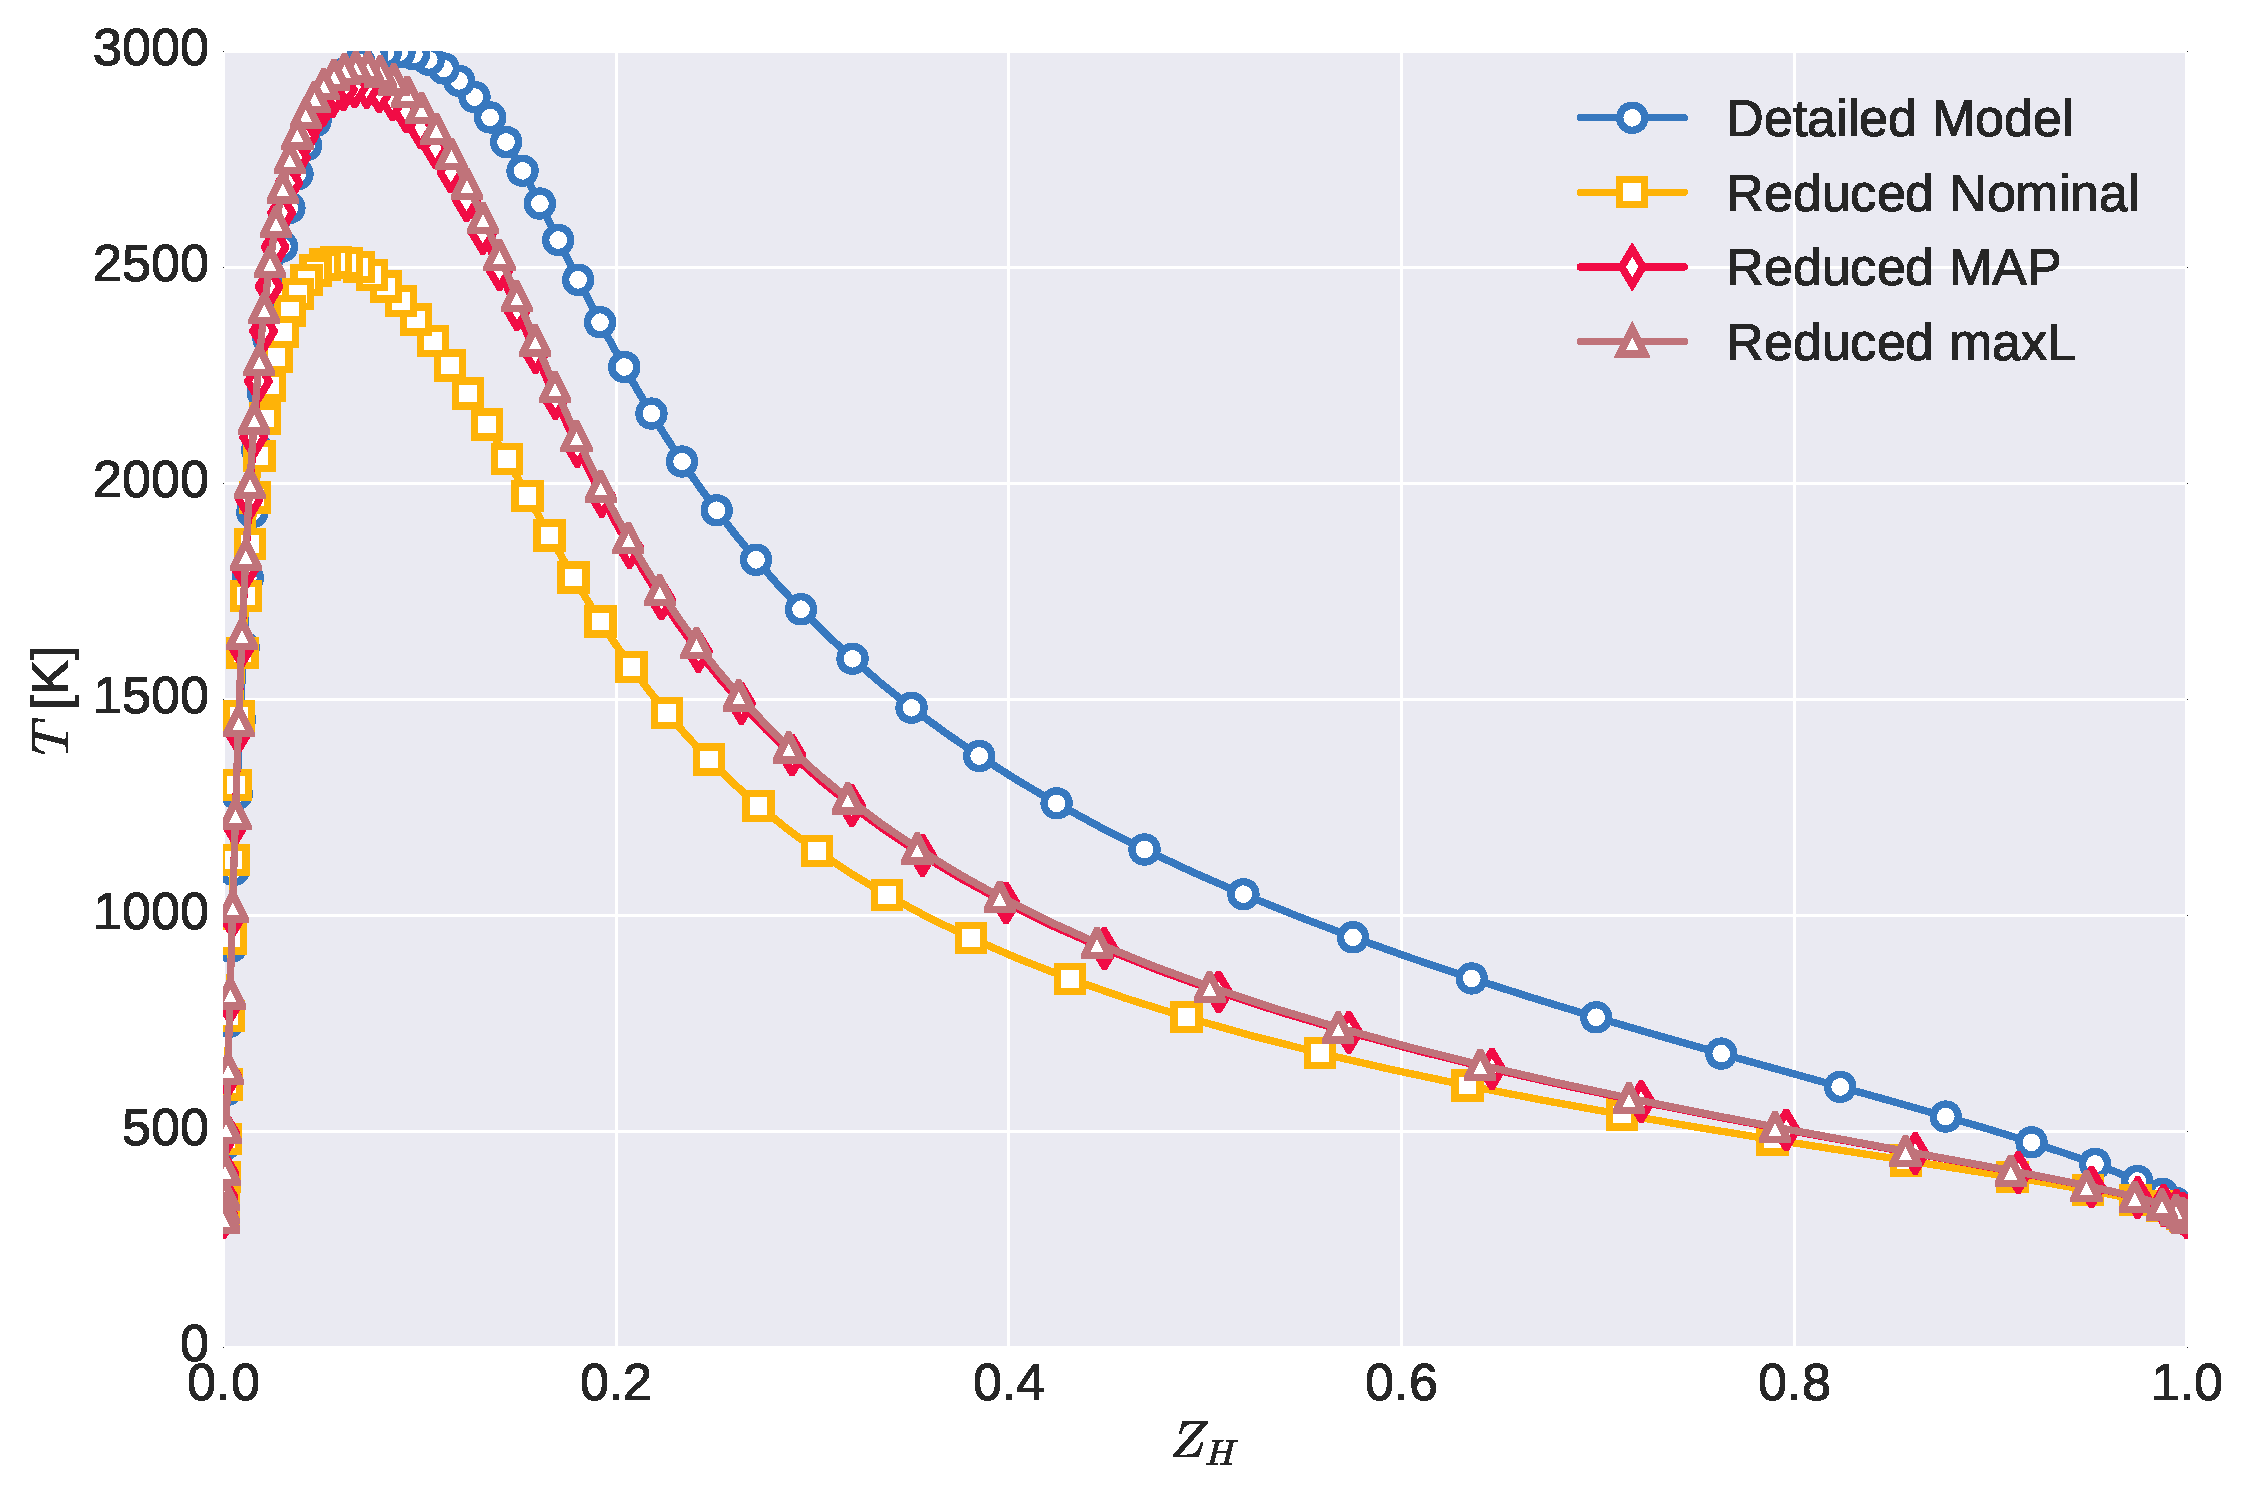
\includegraphics[width=0.7\textwidth]{/h1/dsondak/Research-Notebook/figures/2016/July/T_Z.pdf}
  \caption{Temperature as a function of mixture fraction.}
  \label{fig:T_Z}
\end{figure}
\begin{figure}[h!]
  \centering
  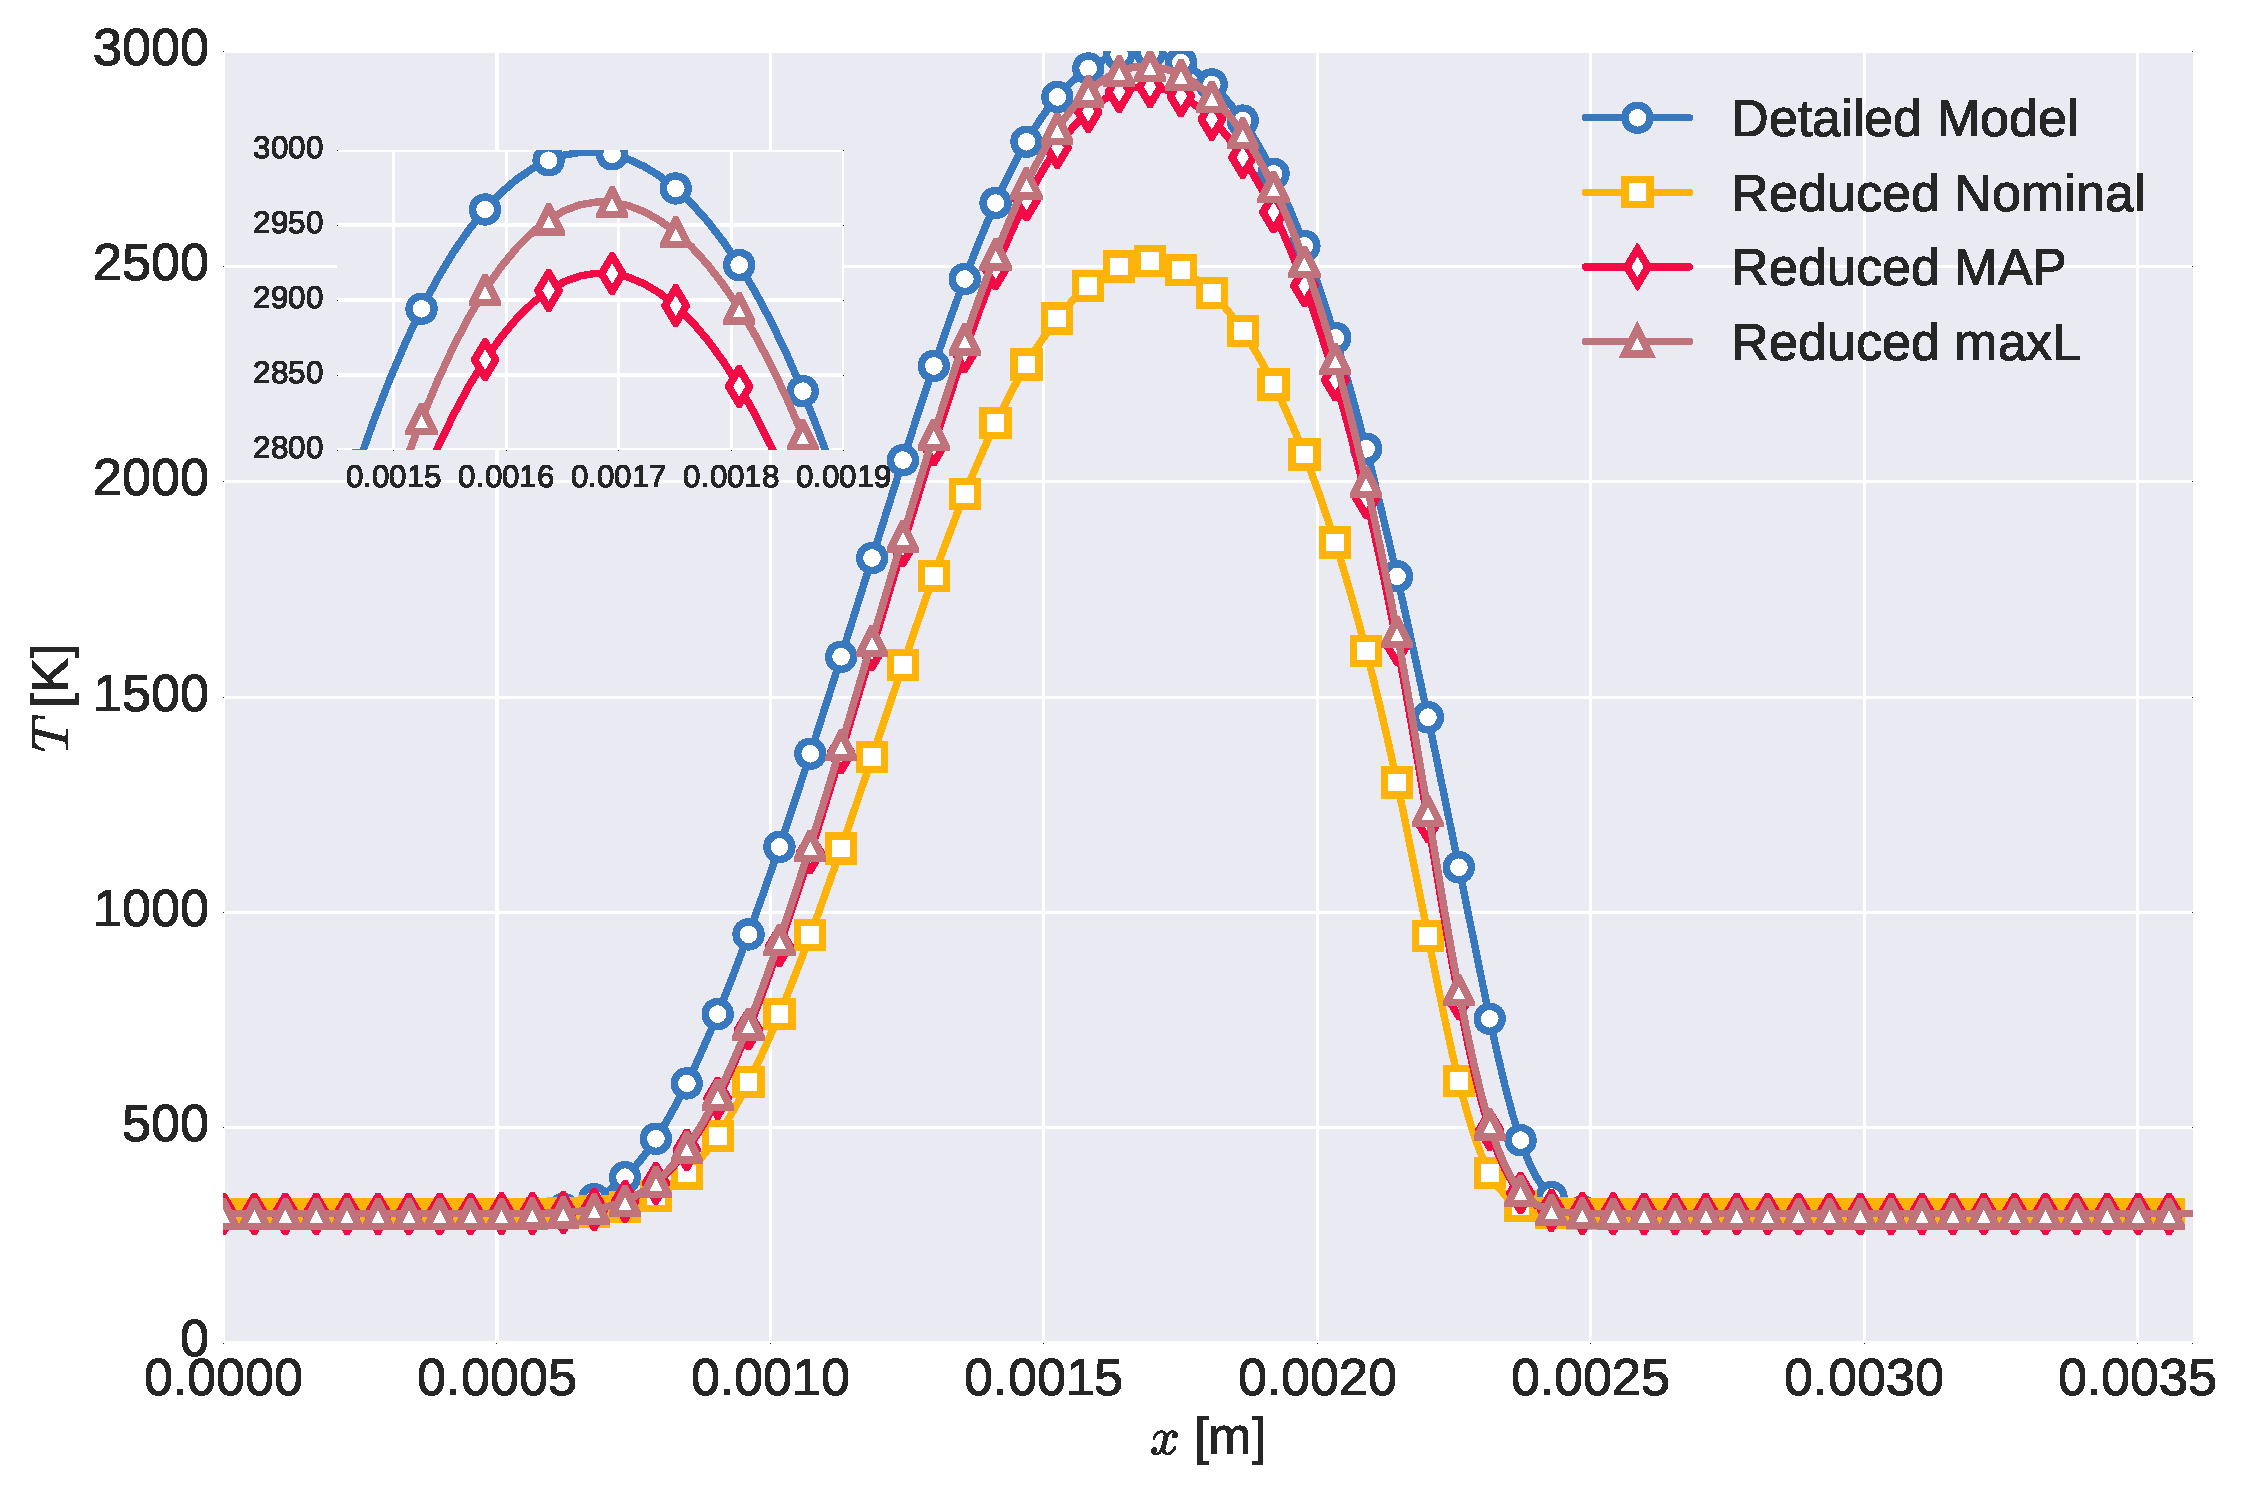
\includegraphics[width=0.7\textwidth]{/h1/dsondak/Research-Notebook/figures/2016/July/T_x.pdf}
  \caption{Temperature as a function of space.}
  \label{fig:T_x}
\end{figure}
\begin{figure}[h!]
  \centering
  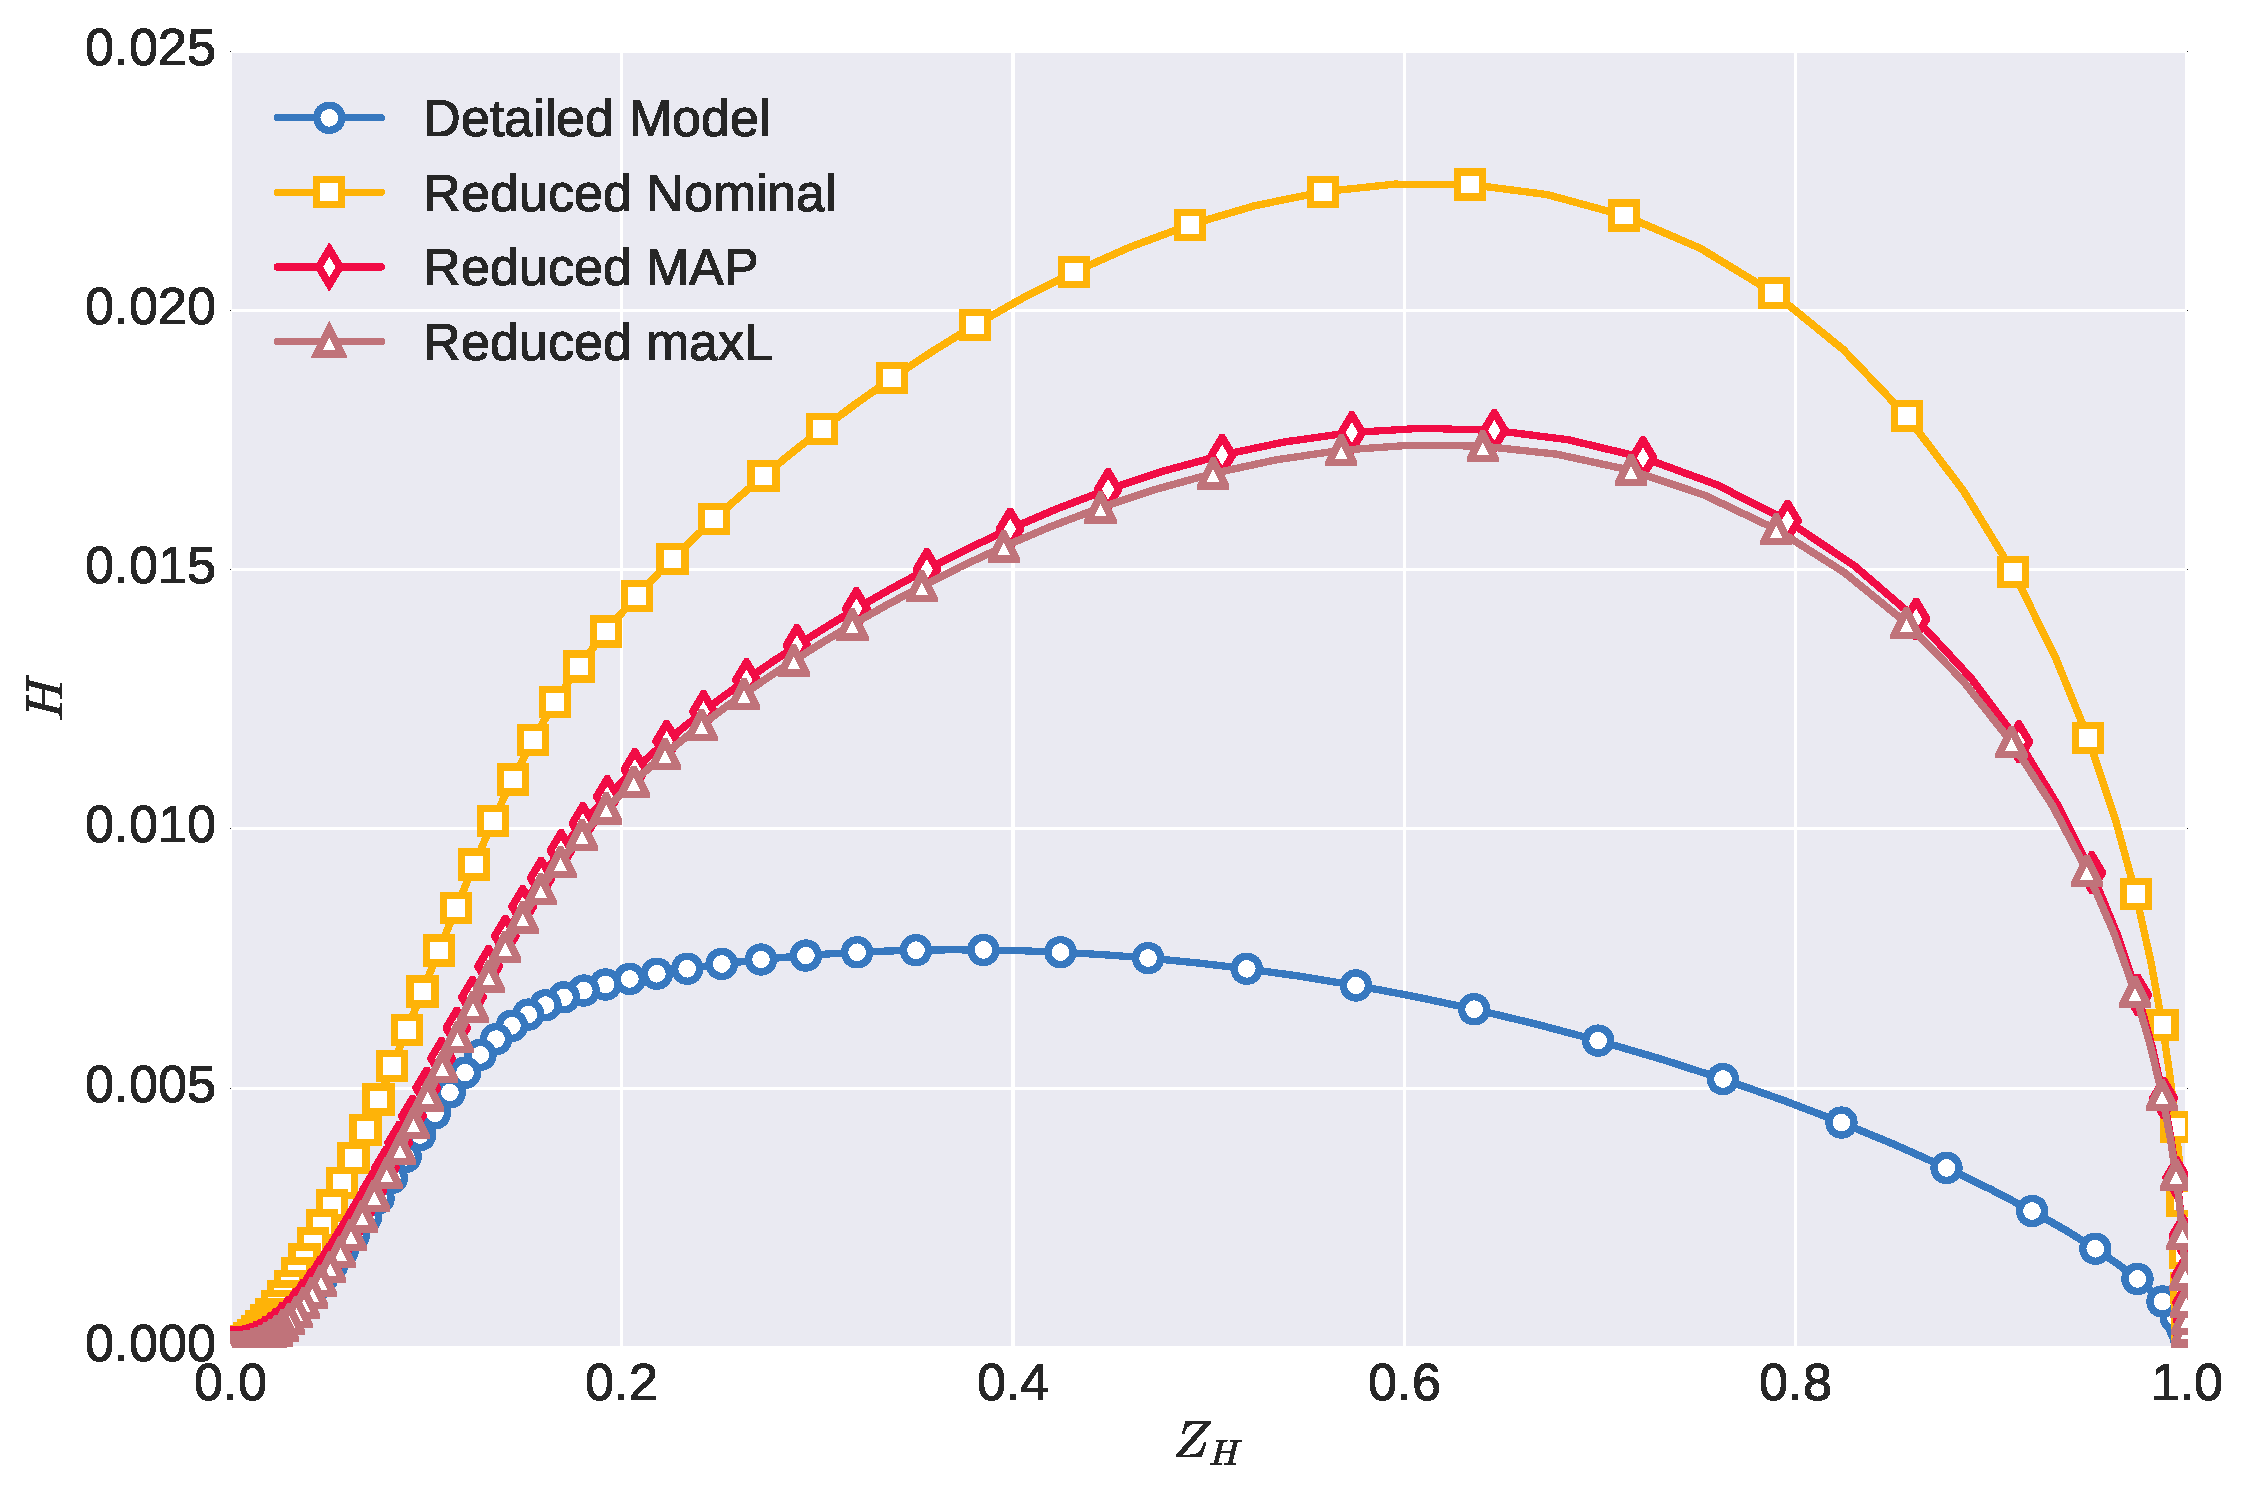
\includegraphics[width=0.7\textwidth]{/h1/dsondak/Research-Notebook/figures/2016/July/H_Z.pdf}
  \caption{Hydrogen as a function of mixture fraction.}
  \label{fig:H2_Z}
\end{figure}
\begin{figure}[h!]
  \centering
  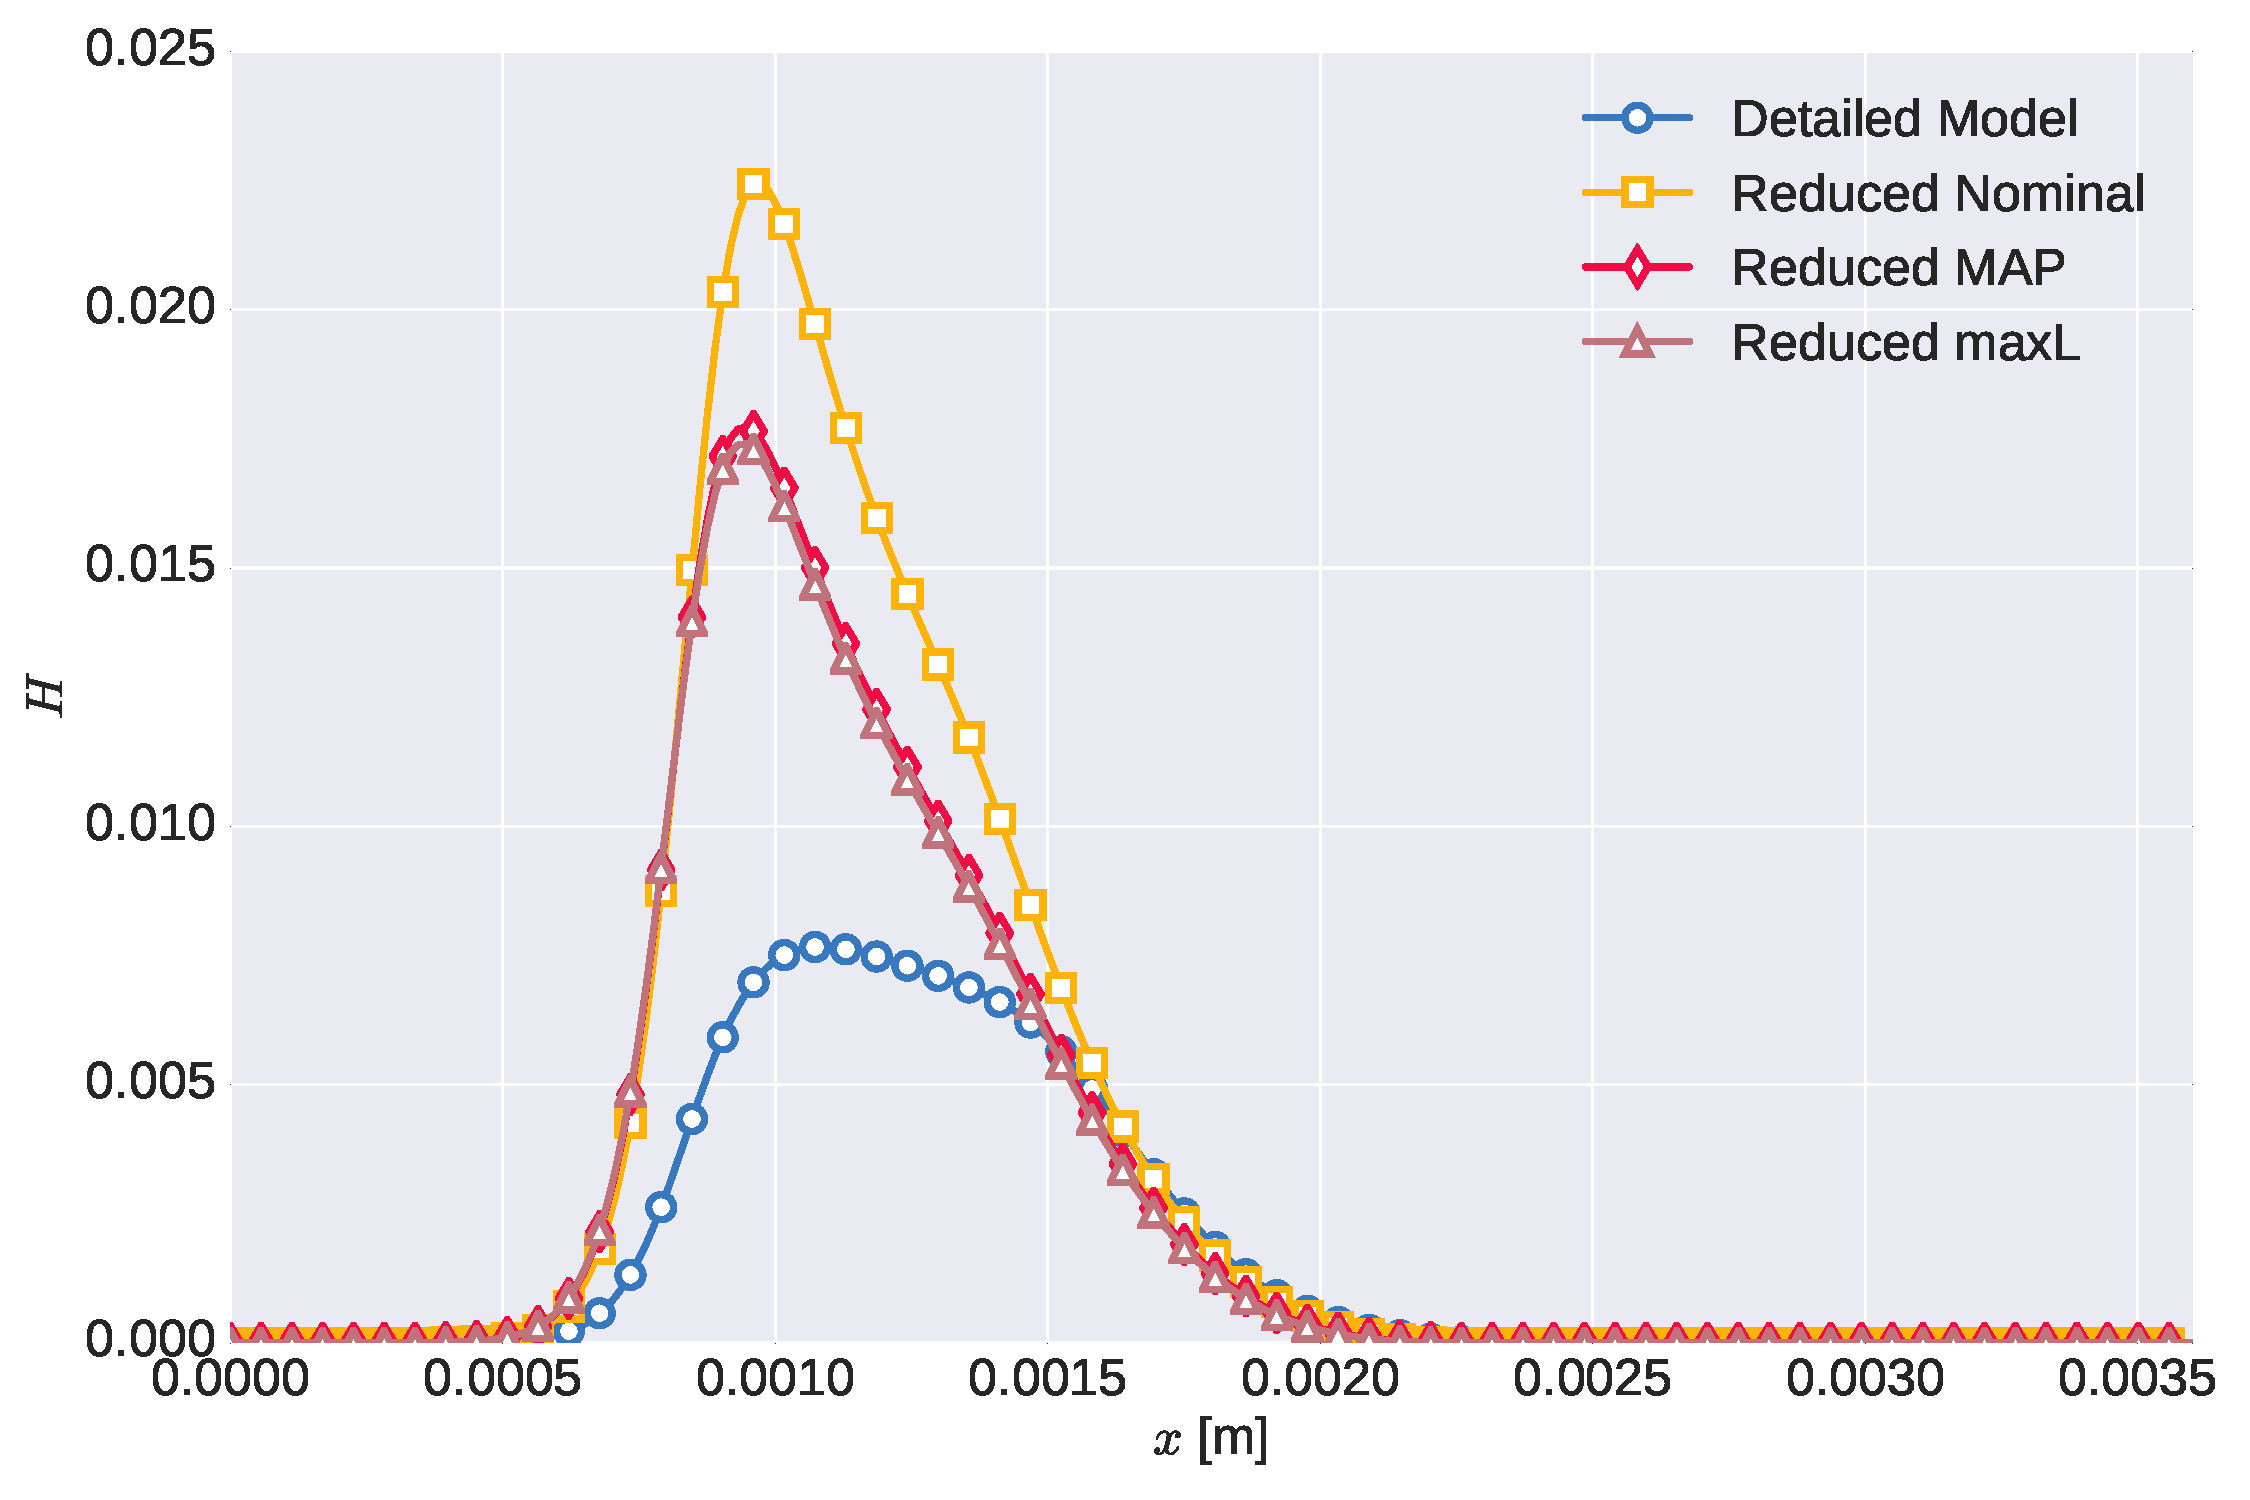
\includegraphics[width=0.7\textwidth]{/h1/dsondak/Research-Notebook/figures/2016/July/H_x.pdf}
  \caption{Hydrogen as a function of space.}
  \label{fig:H2_x}
\end{figure}
The plots of \ce{H} are clearly inadequate by almost any measure.  The plot of temperature with
mixture fraction also appears inadequate.  However, when plotting temperature with space, the results
look pretty good.  Other results indicate that some species are shifted in the domain.  That is, 
the flame location is not correct.  The concentration of \ce{HO2} is horrendously off to the point
where the reduced model predicts non-negligible concentrations while the detailed model predicts 
that \ce{HO2} is a trace species.  A few species, such as \ce{H2O}, \ce{H2} and \ce{O2} are more
or less correct as expected.  To quantify this a bit more, I will run a few samples from the chain
through the diffusion flame to see if I can put some error bars on the plots.  It will be difficult
to do this for the plots with mixture fraction since the mixture fraction will also have error bars.
However, maybe the spatial plots will show some inadequacy.

I propagated $1000$ samples through the diffusion flame and computed the mean and standard deviation
of the temperature at each grid point.  The results are plotted in Figure~\ref{fig:inad_T_x}.
\begin{figure}[h!]
  \centering
  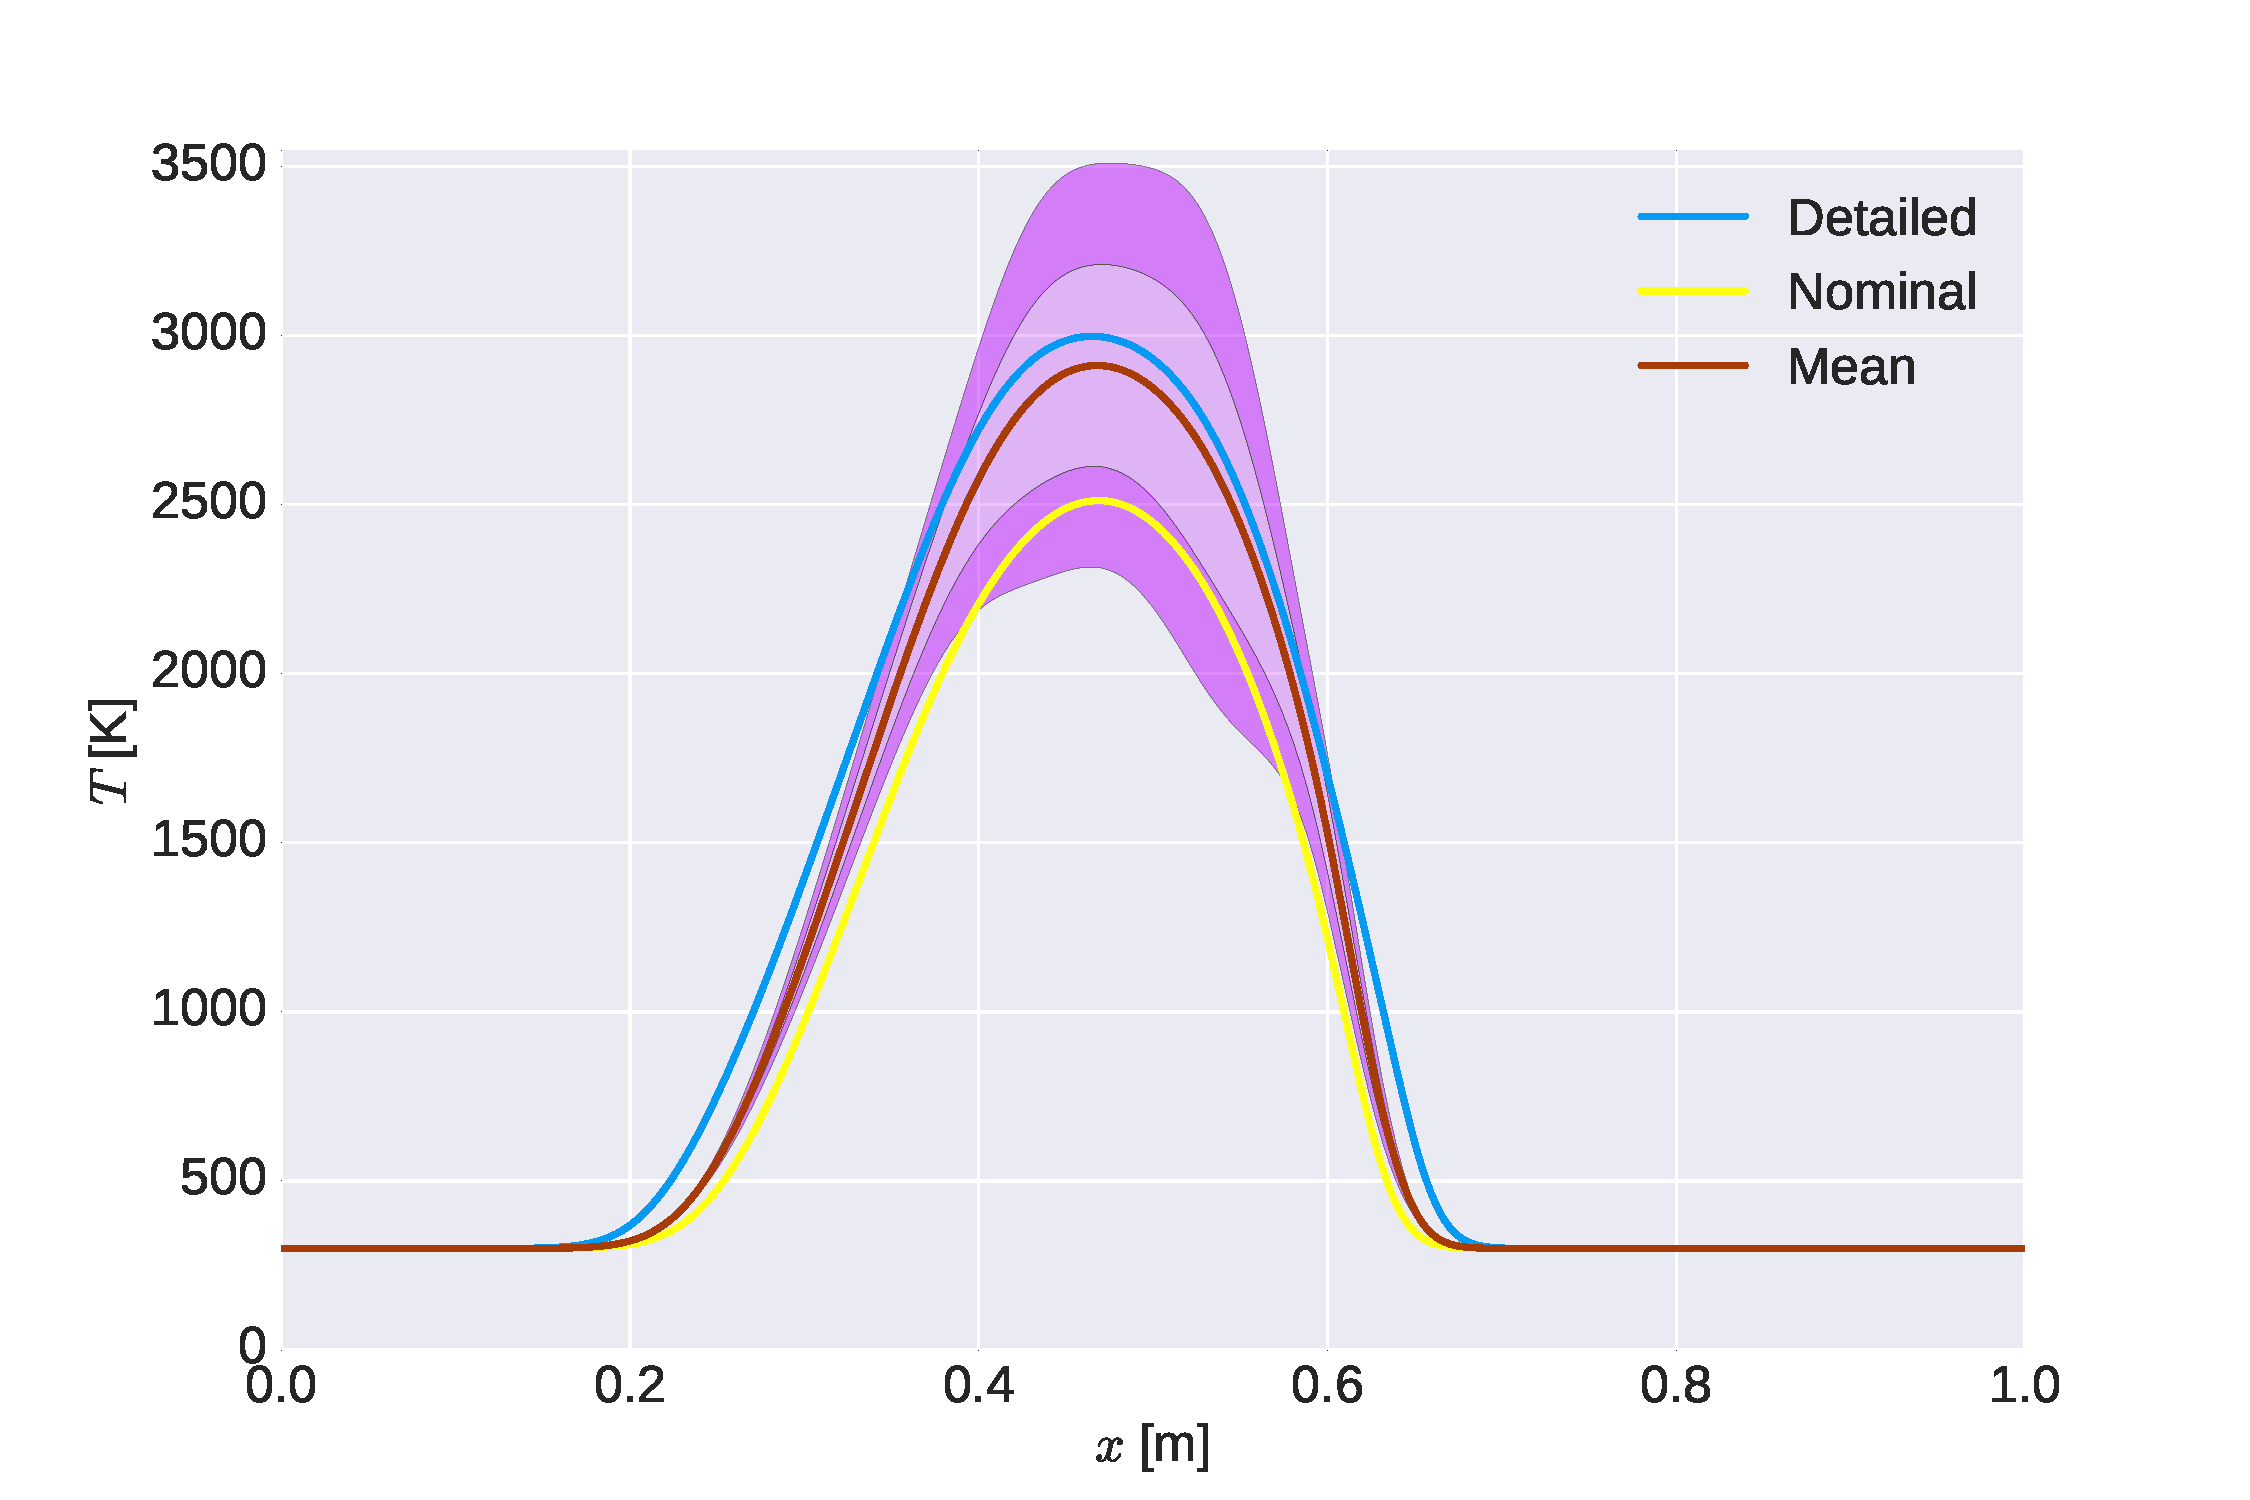
\includegraphics[width=0.7\textwidth]{/h1/dsondak/Research-Notebook/figures/2016/July/inad_T_x.pdf}
  \caption{Inadequacy in temperature profile across the diffusion flame.  Dark shading represents two
           standard deviations while light shading represents one standard deviation.  Most of the
           inadequacy occurs near the boundary of the flame.}
  \label{fig:inad_T_x}
\end{figure}
The calibrated reduced model does quite well at predicting the diffusion flame.  The main inadequacies 
are found near the boundaries of the flame.  Otherwise, the detailed model falls easily within one
standard deviation of the mean.

%----------------------------------------------------------------------------------------

\labday{Friday, 29 July, 2016}

%-----------------------------------------
\experiment{Combustion Model Inadequacy}
\begin{itemize}
  \item Working on APS abtract for Turbulent Combustion session
  \item Found a mistake in Rebecca's formulation.
\end{itemize}

\subexperiment{Chemical Kinetics Inadequacy}
Theorem 3.2 in ~\cite{morrison2016representing} describes how to form a reaction based upon the stochastic operator.  The problem is that the stoichiometric coefficients are not treated correctly in the theorem.  They should enter as exponents, not as prefactors.  I present a description here of a system of reactions induced by the linear part of the stochastic operator.  Recall that the system of equations governing concentrations of species in the zero-D rector is
\begin{align}
  \odeone{\mathbf{x}}{t} = \mathbf{f}\lr{\mathbf{x}} + \mathcal{S}\mathbf{x} + \mathbf{g}\lr{\mathbf{x}} \label{eq:OD-system}
\end{align}
where $\mathbf{x} = \left[x_{1}, \ldots, x_{2}\right]^{T}$ is a vector containing species concentrations.  The $i^{\text{th}}$ component represents species $i$.  The right hand side consists of the chemical mechanism, $f\lr{\mathbf{x}}$, the linear part of the stochastic operator $\mathcal{S}\mathbf{x}$ and the so-called catchall reactions $g\lr{\mathbf{x}}$.  We will not consider the catchall reactions here because their form is not in question at the moment.  In chemical kinetics, the reaction rate for species $k$ given by
\begin{align}
  \dot{\omega}_{k} = \sum_{j=1}^{M}\lr{\nup{kj} - \nur{kj}}r_{j} \label{eq:react_rate}
\end{align}
where the progress rate of reaction $j$ is
\begin{align}
  r_{j} = \frate{j}\prod_{k=1}^{N}{x_{k}^{\nur{kj}}} - \rrate{j}\prod_{k=1}^{N}{x_{k}^{\nup{kj}}}.
\end{align}
Note that we are working with molar concentrations here.  To convert to mass fraction, we would multiply~\eqref{eq:react_rate} by the molecular weight of species $k$.  The classical expression for the forward reaction rate coefficient is the Arrhenius reaction rate
\begin{align}
  \frate{j} = A_{j}T^{b_{j}}\exp\lr{-\frac{E_{j}}{RT}} \label{eq:arrhenius}.
\end{align}
The goal is now to interpret $\mathcal{S}\mathbf{x}$ in terms of the previously described reaction rates.

Note that the contribution to species $k$ from the linear part of the stochastic operator is
\begin{align}
  \lr{\mathcal{S}\mathbf{x}}_{k} = \sum_{j=1}^{N}{s_{kj}x_{j}}. \label{eq:Sx}
\end{align}
Equation~\eqref{eq:Sx} can be interpreted as a reaction rate induced by $N$ reactions of the form
\begin{align}
  \ce{x_{p} ->[$s_{kp}$] x_{k}}, \quad p \neq k
\end{align}
where the reaction rate parameter $\frate{j}$ is just a constant $s_{kj}$.  When $p = k$ a modification must be introduced,
\begin{align}
  \ce{x_{k} ->[$s_{kk}$] 2 x_{k}}.
\end{align}

To clarify this formulation, we do a couple of examples.  In the \ce{H2}-\ce{O2} example, the linear part of the stochastic operator contributes to atomic hydrogen via
\begin{align}
  \odeone{\left[\ce{H}\right]}{t} = f_{\ce{H}}\lr{\mathbf{x}} + s_{57}\left[\ce{OH}\right] + s_{58}\left[\ce{HO2}\right] + s_{59}\left[\ce{H2O}\right].
\end{align}
The set of reactions is therefore
\begin{align}
  \ce{OH ->[s_{57}] H} \\
  \ce{HO2 ->[s_{58}] H} \\
  \ce{H2O ->[s_{59}] H}.
\end{align}
The progress rates become
\begin{align}
  r_{1} = s_{57}\left[\ce{OH}\right] \\
  r_{2} = s_{58}\left[\ce{HO2}\right] \\
  r_{3} = s_{59}\left[\ce{H2O}\right]. 
\end{align}
Therefore, the reaction rate for the linear part of the operator is
\begin{align}
  \dot{\omega}_{\ce{H}} = s_{57}\left[\ce{OH}\right] + s_{58}\left[\ce{HO2}\right] + s_{59}\left[\ce{H2O}\right].
\end{align}

The contribution to hydrogen is more involved.  It is
\begin{align}
  \odeone{\left[\ce{H2}\right]}{t} = f_{\ce{H2}}\lr{\mathbf{x}} + s_{31}\left[\ce{H^{\prime}}\right] + s_{33}\left[\ce{H2}\right] + s_{35}\left[\ce{H}\right] + s_{37}\left[\ce{OH}\right] + s_{38}\left[\ce{HO2}\right] + s_{39}\left[\ce{H2O}\right].
\end{align}
The corresponding reaction set is
\begin{align}
  \ce{H^{\prime} ->[s_{31}] \ce{H2}} \\
  \ce{H          ->[s_{35}] \ce{H2}} \\
  \ce{OH         ->[s_{37}] \ce{H2}} \\
  \ce{HO2        ->[s_{38}] \ce{H2}} \\
  \ce{H2O        ->[s_{39}] \ce{H2}}
\end{align}
and
\begin{align}
  \ce{H2 ->[s_{33}] \ce{2H2}}
\end{align}
with reaction progress rates
\begin{align}
  r_{1} = s_{31}\left[\ce{H^{\prime}}\right] \\
  r_{2} = s_{33}\left[\ce{H2}\right] \\
  r_{3} = s_{35}\left[\ce{H}\right] \\
  r_{4} = s_{37}\left[\ce{OH}\right] \\
  r_{5} = s_{38}\left[\ce{HO2}\right] \\
  r_{6} = s_{39}\left[\ce{H2O}\right].
\end{align}
We are then able to recover the reaction rate induced for \ce{H2} by the linear part of the stochastic operator.  Implementation of this formulation in the \textt{XML} input format will be a challenge.
